\documentclass{article}
\usepackage[utf8]{inputenc}
\usepackage{graphicx}
\usepackage[super,negative]{nth}
\usepackage{longtable}
\usepackage{multirow}
\usepackage{fancyhdr}
\usepackage{float}
\usepackage{subfig}
\usepackage{color, soulutf8}
\usepackage{graphicx}
\usepackage{grffile}

\usepackage{hyperref}
\hypersetup{
	colorlinks=true,
	linkcolor=black,
	filecolor=black,      
	urlcolor=black,
}

\usepackage[dvipsnames]{xcolor}
\usepackage{listings}

\renewcommand{\thefigure}{\arabic{section}.\arabic{figure}}
\newcommand\goal[1]{\item[{[G#1]}] }
\newcommand\requirement[1]{\item[{[R#1]}] }
\newcommand\assumption[1]{\item[{[A#1]}] }
\newcommand\usecase[1]{ [UC#1] }

\begin{document}
	\begin{titlepage}
		
		\centering
		\vspace*{0.7 cm}
		
\includegraphics[scale = 0.7]{images/PolimiLogo.png}\\[1 cm]
		\textsc{\large Dipartimento di Elettronica, Informazione e Bioingegneria}\\[2 cm]
		
		\rule{\linewidth}{0.2 mm} \\[0.5 cm]
		{\huge \bfseries Design Document (DD)}\\
		\rule{\linewidth}{0.2 mm} \\[1.5 cm]
		
		\textsc{\Large SafeStreets}\\[0.5 cm]
		\textsc{\large - v1.0 -}\\[1 cm]
		
		\begin{minipage}{\textwidth}
			\begin{flushleft} \large
				\emph{Authors:}\\
				\textbf{Quacquarelli} Sebastiano \hfill 945071 \\
				\textbf{Ricchiuti} Simone \hfill 945613  \\
				\textbf{Sala} Nicolò \hfill 945898  \\[2 cm]
			\end{flushleft}
		\end{minipage}\\[2 cm]
		
		{\large December \nth{9} , 2019}\\[2 cm]
		
	\end{titlepage}
	
	\pagenumbering{roman}
	\tableofcontents
	\clearpage
	\newpage
	\pagenumbering{arabic}
	\setcounter{page}{1}
	
	\section{Introduction}
		\subsection{Purpose}
		The main aspects of SafeStreets system are presented in the RASD document (see References section). The purpose of this document is to describe in a more detailed way the technical aspects regarding architectural and design choices for SafeStreets components.\\\\
		More precisely, the document presents:
		\begin{itemize}
			\item Overview of the high level architecture;
			\item The main components, their interfaces; 
			\item The runtime behaviour; 
			\item The design patterns;
			\item Additional details about user interface;
			\item A mapping of the requirements on the architecture's components;
			\item Implementation, integration and testing plan;

		\end{itemize}
		\subsection{Scope}
		In this section is shortly summarised what is already defined in a more detailed way in the \textit{Scope} section of the RASD document.\\
		SafeStreets scope is to give the opportunity to report traffic violations by users and eventually to let them be managed by a competent authority in an easy way. Basically users can simply open the SafeStreets Application on their smartphones and immediately take a picture of the traffic violation to report. Including a few more information, the report is done and is ready to be sent to SafeStreets system.\\
		On the other hand, authorities in collaboration with SafeStreets can check violation reports on their SafeStreets Authority Edition (desktop dedicated application).\\
		Evaluating reports, authorities can eventually define them consistent or not and, if consistent evaluated, they fine the offender reported.\\
		These ones are the basic functionalities offered by SafeStreets but also other ones are offered to individuals:
		\begin{itemize}
			\item Users can browse the map to know statistics about traffic violations sent to SafeStreets and their status (confirmed or not by authorities);
			\item Authorities can browse map such as users but including access also to sensitive information such as license plates included in reports;
			\item Authorities can access to advanced statistics such as filtering results to return the most egregious offender;
			\item Authorities can also send to SafeStreets some information about accidents in order to enrich SafeStreets database. It is important because authorities can receive suggestions from SafeStreets system to improve the security of streets according to violations and accidents occurred in a defined area.
		\end{itemize}
		\subsection{Definitions, Acronyms, Abbreviations}
		\subsubsection{Definitions}
		\begin{itemize}
			\item \textbf{Operative area}: the geographic area in which an authority retains control and actually works.
			\item \textbf{Registered authority}: an authority that decided to participate in SafeStreets initiative and that installed in its head office SafeStreets AE, a particular version of the application that provides some features not available to common users (for example, the possibility to rate the traffic violation reports collected by SafeStreets).
			\item \textbf{Report image}: it is the image acquired through the SafeStreets app. It is obligatorily associated with a valid report.
			\item \textbf{Report timeout}: it is the timeout started when SafeStreets app acquires the report image. If the user doesn't complete the completion of the report by the deadline of this timeout, the report is considered invalid.
			\item \textbf{SafeStreets}: it is the crowdfunding app subject of this document.
			\item \textbf{SafeStreets application}: it is the application used by users, installed on their smartphone.
			\item \textbf{SafeStreets Authority Edition}: it is the application used by authorities, installed on computers in their station.
			\item \textbf{SafeStreets Client}: a generic way to point out the SafeStreets App or the SafeStreets Authority Edition.
			\item \textbf{Traffic violation report}: it is the message that SafeStreets collects through its app from users who want to report an alleged violation. It is often abbreviated as "report".
			\item \textbf{Individual}: A generic user or authority.
		\end{itemize}
		\subsubsection{Acronyms}
		\begin{itemize}
			\item \textbf{AE} \label{AE}: SafeStreets Authority Edition.
			\item \textbf{GUI} \label{GUI}: Graphic User Interface.
			\item \textbf{HTTP} \label{HTTP}: Hypertext Transfer Protocol.
			\item \textbf{MVC} \label{MVC}: Model-View-Controller design pattern.
			\item \textbf{OCR} \label{OCR}: Optical Character Recognition.
			\item \textbf{RASD} \label{RASD}: Requirement Analysis and Specification Document.
			\item \textbf{REST} \label{REST}: REpresentational State Transfer.
			\item \textbf{URI} \label{URI}: Universal Resource Identifier.

		\end{itemize}
		\subsubsection{Abbreviations}
		\begin{itemize}
			\item {[DB]}: Database.
			\item {[Rn]}: n\textsuperscript{th} functional requirement.

		\end{itemize}
		\subsection{Revision history}
			\begin{table}[h]
				\centering
				\begin{tabular}{c c c}
					\hline
					\textbf{Version} & \textbf{Last update} & \textbf{Comments} \\ 
					\hline
					1.0 &  \nth{9} December, 2019  & \\
					\hline
				\end{tabular}
				\caption{Revision history}
				\label{fig:Revision history}
			\end{table}
		\subsection{Document structure}
			In this part it is shown how the document has been divided. For each chapter, is given a short description:
			\begin{itemize}
				\item \textit{Chapter 1} gives an introduction of the design document. It contains the purpose of the document and the scope of the SafeStreets system, as well as some abbreviations in order to provide a better understanding of the document to the reader.
				\item \textit{Chapter 2} is the core section of the design document and it deals with the architectural design of the application. It gives an overview of the architecture and it also contains the most relevant architecture views: 
				\begin{itemize}
					\item High‐level components and their interactions;
					\item Component view;
					\item Deployment view;
					\item Component interfaces;
					\item Runtime view. 
				\end{itemize}
			  	Some of the used architectural designs and designs patterns are also presented here, with an explanation of each one and the purpose of their usage.				
				\item \textit{Chapter 3} refers to the mockups already presented in the RASD document including some more detailed versions of them such as interaction diagrams.
				\item \textit{Chapter 4} explains how the requirements that were defined in the RASD are now assigned to the design elements defined in this document.
				\item \textit{Chapter 5} presents the implementation, integration and test plan. It specifies how the different components of the application are integrated with each other and the testing strategy.				
				\item \textit{Chapter 6} shows the effort spent by each group member while working on this document.
				\item \textit{Chapter 7} simply includes the references.
			\end{itemize}
		
	\clearpage
	\section{Architectural design}
		\subsection{Overview}
		In this section is defined the high-level architecture of SafeStreets system.\\ 
		Figure \ref{fig:hinteraction_diagram} represents the high level interaction between the main parts of SafeStreets' structure.
		\begin{figure}[H]
			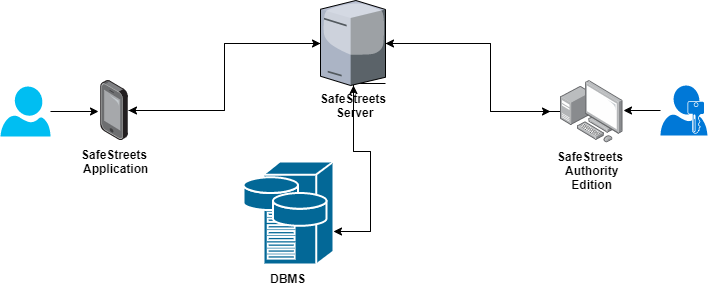
\includegraphics [scale=0.5] {diagrams/high-interaction.png}
			\caption[High-Level Interaction]{High-Level Interaction diagram}
			\label{fig:hinteraction_diagram}
		\end{figure}
		The figure describes how individuals interact with SafeStreets. Only one user is represented on the left and only one authority on the right, but this is only made to define clearly interactions. The real system is actually composed by multiple individuals.\\
		Basically everyone can download the SafeStreets application on his smartphone and can be an \textit{user}. On the other hand the Authority Edition is distributed by SafeStreets only to certificated \textit{authorities} that wants to collaborate with it. 
		\begin{figure}[H]
			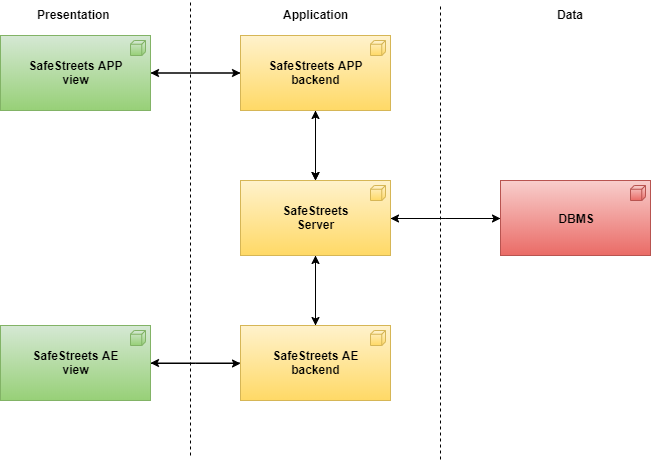
\includegraphics [scale=0.5] {diagrams/system_overview.png}
			\caption[High-Level Layers]{High-Level layers}
			\label{fig:hlayers}
		\end{figure}
		In figure \ref{fig:hlayers}	are shown the three software logic layers by which the system is defined.\\
		\\
		The \textit{Presentation layer} contains the presentation logic of the system. It includes the two views addressed to different kind of SafeStreets clients.\\ The SafeStreets App is addressed to everyone that is interested in SafeStreets and uses its services through the smartphone application.\\
		The SafeStreets Authority Edition (AE) is addressed to certified authorities collaborating with SafeStreets that have received from SafeStreets the desktop application.\\
		\\
		The \textit{Application layer} contains the application logic of the system. Basically it is the layer in which all functionalities are implemented.\\
		This layer contains the SafeStreets App back-end, the SafeStreets AE back-end and the SafeStreets Server. The two back-ends communicate only with the server. This is important because only the server can exchange messages with the database system of the data layer, ensuring an highest level of security not allowing individuals to access directly to sensitive data.\\
		\\
		The \textit{Data layer} simply contains the Data Management System, that collects and execute queries from relational databases. All the queries results are sent only to the SafeStreets server.
		
		\subsection{Component view}
		Figure \ref{fig:component_diagram} represents all the components of SafeStreets ecosystem.\\
		The diagram focuses on the applicative layer: the presentation layer is described in the section "User interfaces" of the RASD and deepened in section 3 of this document.\\
		The diagram underlines that the clients, SafeStreets app and SafeStreets AE, are not thin: they include part of the application logic.\\
		
		\begin{figure}[H]
			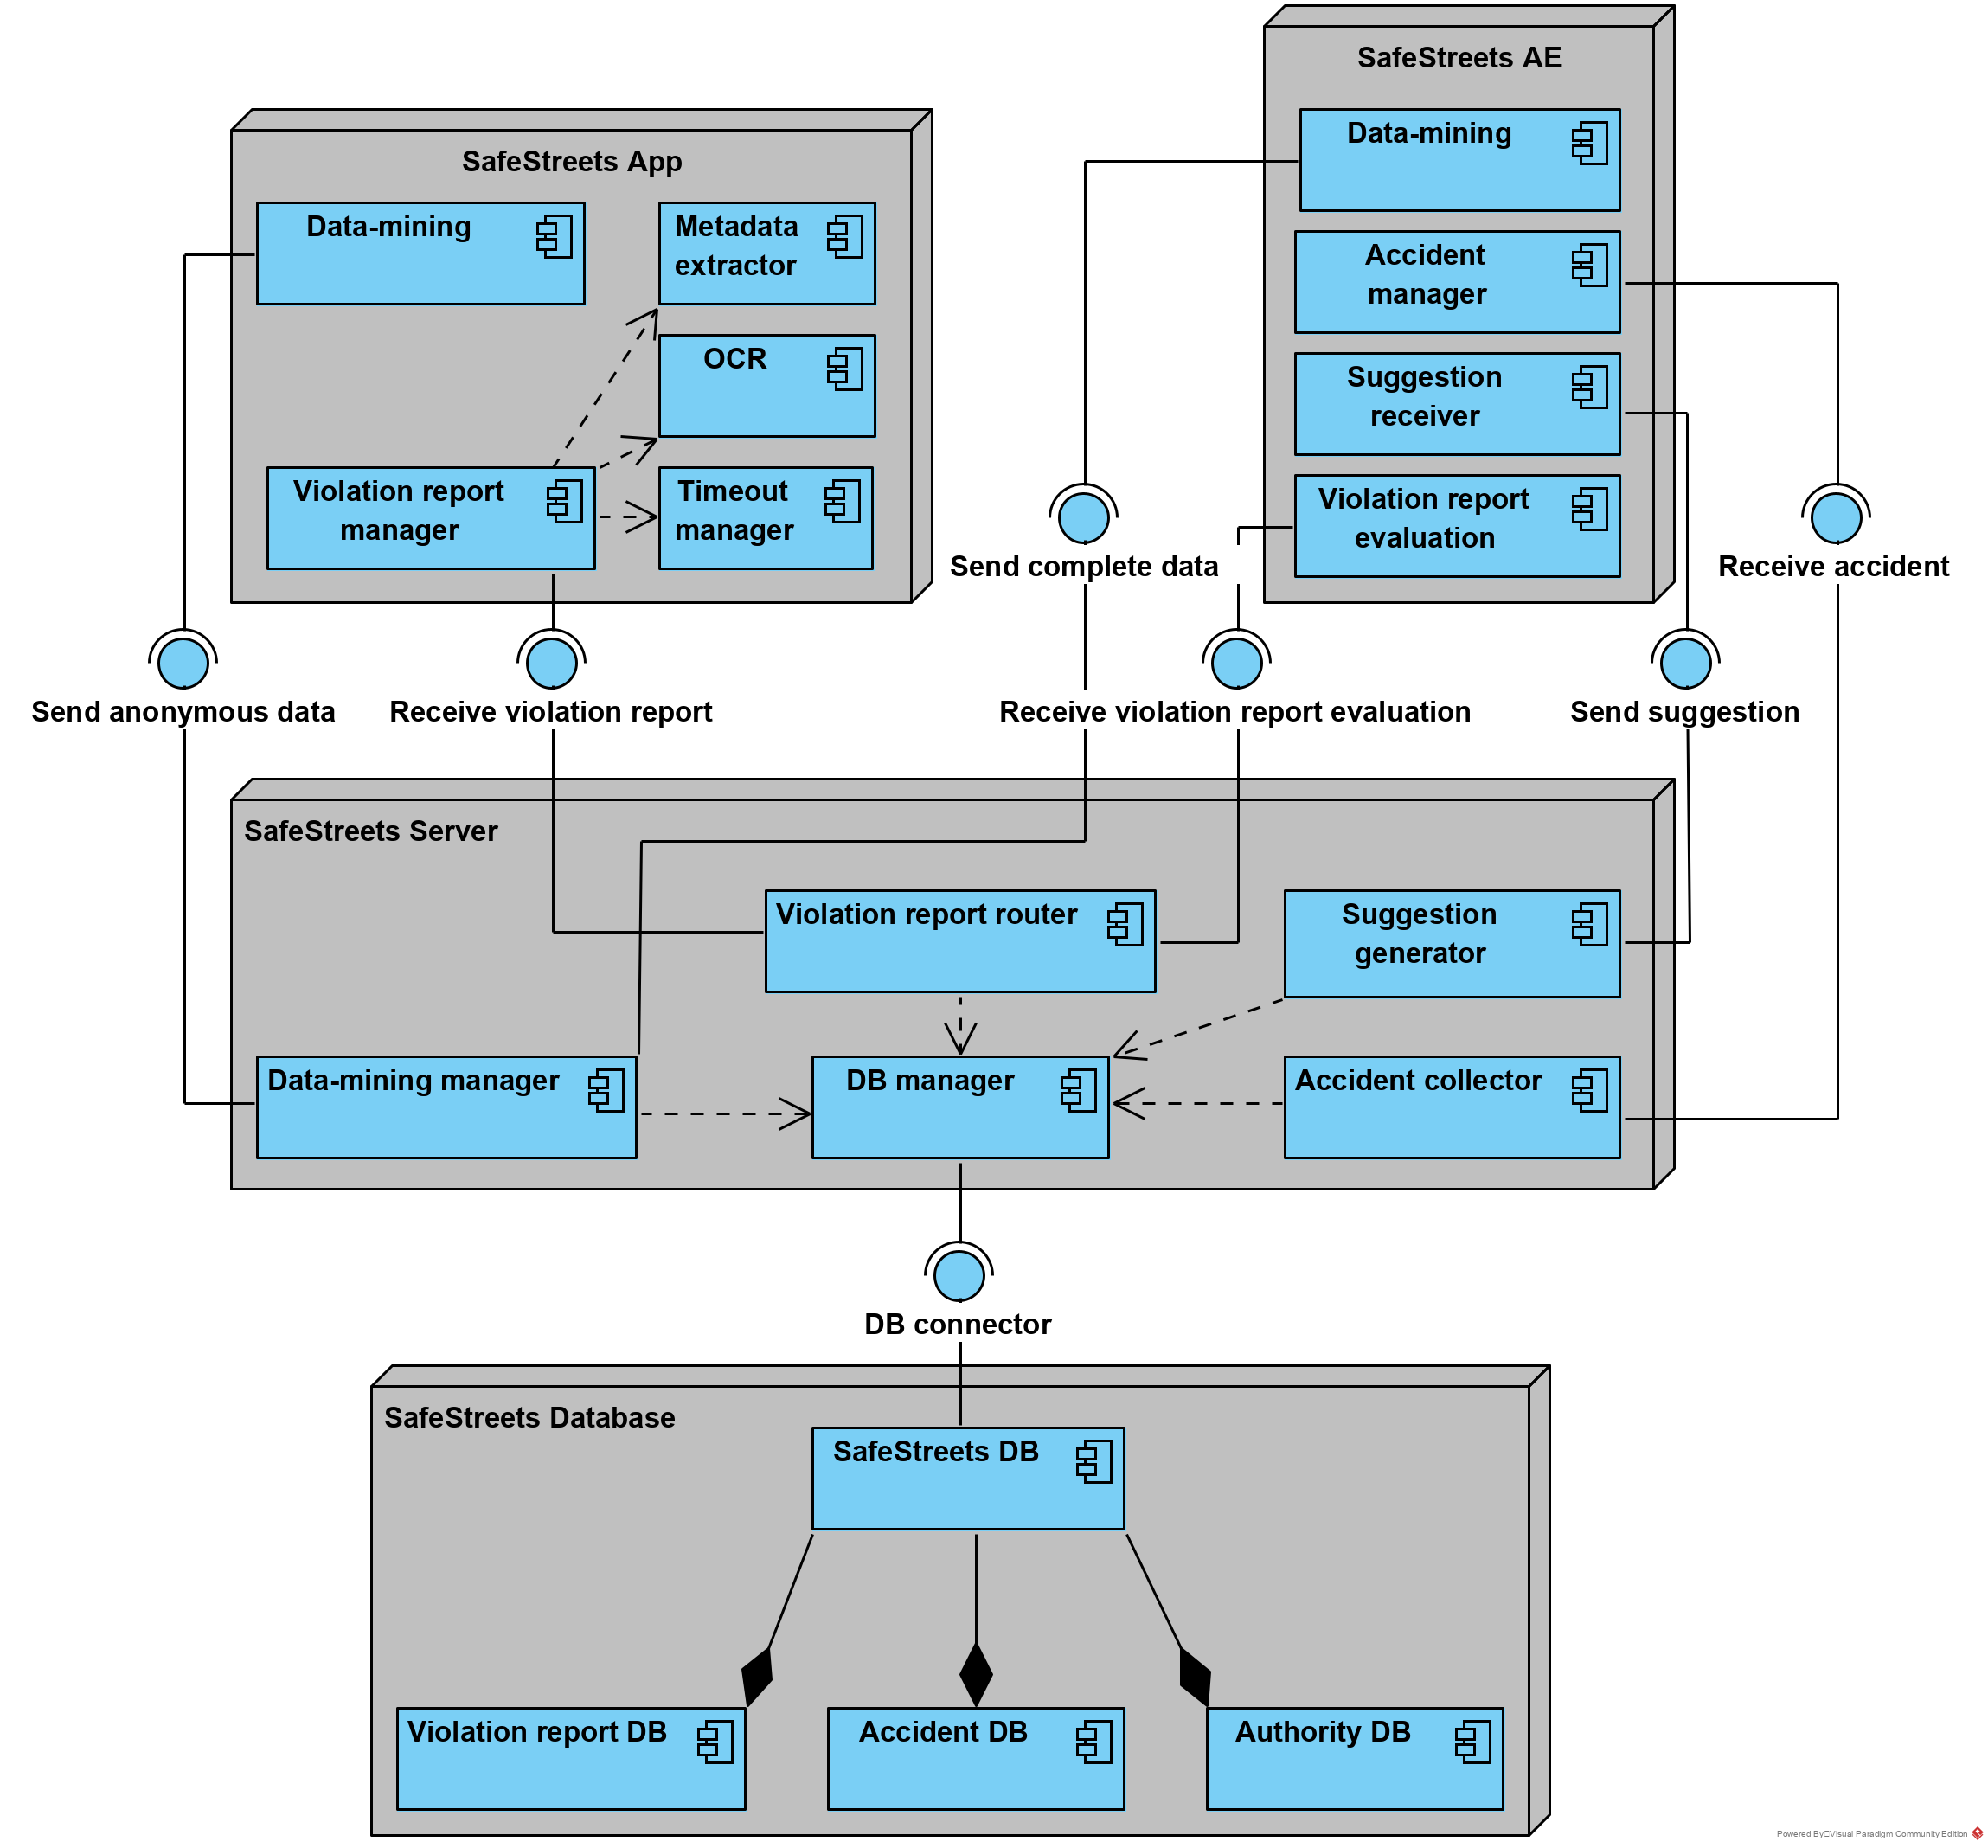
\includegraphics [scale=0.75] {diagrams/component_diagram.png}
			\caption[Component diagram]{Component diagram}
			\label{fig:component_diagram}
		\end{figure}
		
		\clearpage
		For each component of each node, a description of its role is given.
		
		\subsubsection{SafeStreets App components}
		\begin{itemize}
			\item \textbf{Violation report manager}\\
			It deals with the management of a request for a violation report. First of all, it manages the acquisition of the reporting image: it automatically retrieves information about date, time and position. Afterwards, it forwards the image to the license plate recognition algorithm (OCR). If the algorithm returns a valid license plate and the user confirms the request by the deadline of the report timeout, then the violation report manager sends such report to SafeStreets Server through the "violation report" interface.
			\item \textbf{User data-mining}\\
			This component provides data-mining and statistical survey capabilities to SafeStreets App. Remember that SafeStreets App doesn't receive information considered private from the server, in particular it doesn't receive the license plates associated to violations or accidents. The component retrieves information from the server through the "anonymous data" interface.
			\item \textbf{OCR}\\
			This is the software used in order to retrieve a valid license plate from the reporting image. When it receives an image from the violation report manager, it looks for a valid license plate into the image, then returns an error message or the license plate found.
			\item \textbf{Timeout manager}\\
			It manages the report timeout. When the user starts a new violation report request, a timeout starts: if the timeout ends, the timeout manager sends a message to the violation report manager in order to cancel the current violation report request.
		\end{itemize}
		\subsubsection{SafeStreets AE components}
		\begin{itemize}
			\item \textbf{Violation report evaluator}\\
			This component receives violation reports from the server, via the "violation report" interface. After that, it manages the evaluation of the same by the authority. Once the evaluation has taken place, the violation report evaluator sends the result to the server through the aforementioned interface.
			\item \textbf{Authority data-mining}\\
			This component provides data mining and statistical survey capabilities to SafeStreets AE. Remember that SafeStreets AE can also retrieve information about the license plates linked to accidents and violations. The component retrieves information from the server through the "complete data" interface.
			\item \textbf{Suggestion receiver}\\
			It waits for suggestions from the SafeStreets Server, listening the "suggestion" interface. Then it forwards the information to the view.
			\item \textbf{Accident manager}\\
			It manages the forwarding of incident-related information from an authority to SafeStreets Server. It ensures that the reporting of the accident is accompanied by all the data deemed necessary (see RASD, 3.2.1 for more details), after which it forwards the same to the server through the "accident" interface.
		\end{itemize}
		\subsubsection{SafeStreets Server components}
		\begin{itemize}
			\item \textbf{Violation report router}\\
			It passes violation reports received from users to the database. Also, it routes them to the authorities through the "violation report evaluation" interface, so they can be evaluated. The router follows a precise routing policy: it reads the position associated with the violation report, after which it consults the authority database: if there is an authority with has "municipal" jurisdiction for that area, the report is forwarded to it. Otherwise, an authority with "provincial" competence is sought for that area. If this is not the case, an authority with "state" jurisdiction is sought. If no authority can handle the validation of the report, it is not forwarded to any authority.
			\item \textbf{Data-mining manager}\\
			This component handles data requests from SafeStreets clients. In particular, it deals with extracting the data requested from the SafeStreets database, through the DB manager, filtering such data according to the authorizations of visibility available to the applicant. If the applicant is an authority, it can view all the data; if you are a user, the license and image information is deleted before sending it through the "anonymous data" interface.
			\item \textbf{Suggestion generator}\\
			When SafeStreets Server receives a new confirmation of violation or a new incident report, it is also received by this component, which compares the newly obtained data with those already saved in the database. Depending on a table of which it is available, it can generate advice to be sent to the authorities in order to avoid the repetition of certain dangerous situations, through the "suggestions" interface.
			\item \textbf{Accident collector}\\
			This component listens for new incident reports through the "accident" interface. The correctness of these reports has already been confirmed by SafeStreets AE, so it is only necessary to send the new data to the DB manager, so that they are saved in the database.
			\item \textbf{DB manager}\\
			It manages the interaction between SafeStreets Server and SafeStreets Database. All the components of the server that wants to interact with the database has to pass through this component. This means that in the event of updates to the structure or operation of the database, only the DB manager may need to be updated, guaranteeing better independence between the server and the database.
		\end{itemize}
		\subsubsection{SafeStreets Database components}
		The database stores all the information used by SafeStreets ecosystem. It is composed by three sub-databases, whose role can be easily understood from their name: \textbf{Violation report DB}, \textbf{Accident DB} and \textbf{Authority DB}.
		
		\clearpage
		\subsection{Deployment view}
		In this section are defined the devices and the environments in which the three layers defined in the chapter 2.1 are concretely realized.
		
		\begin{figure}[H]
			\centering
			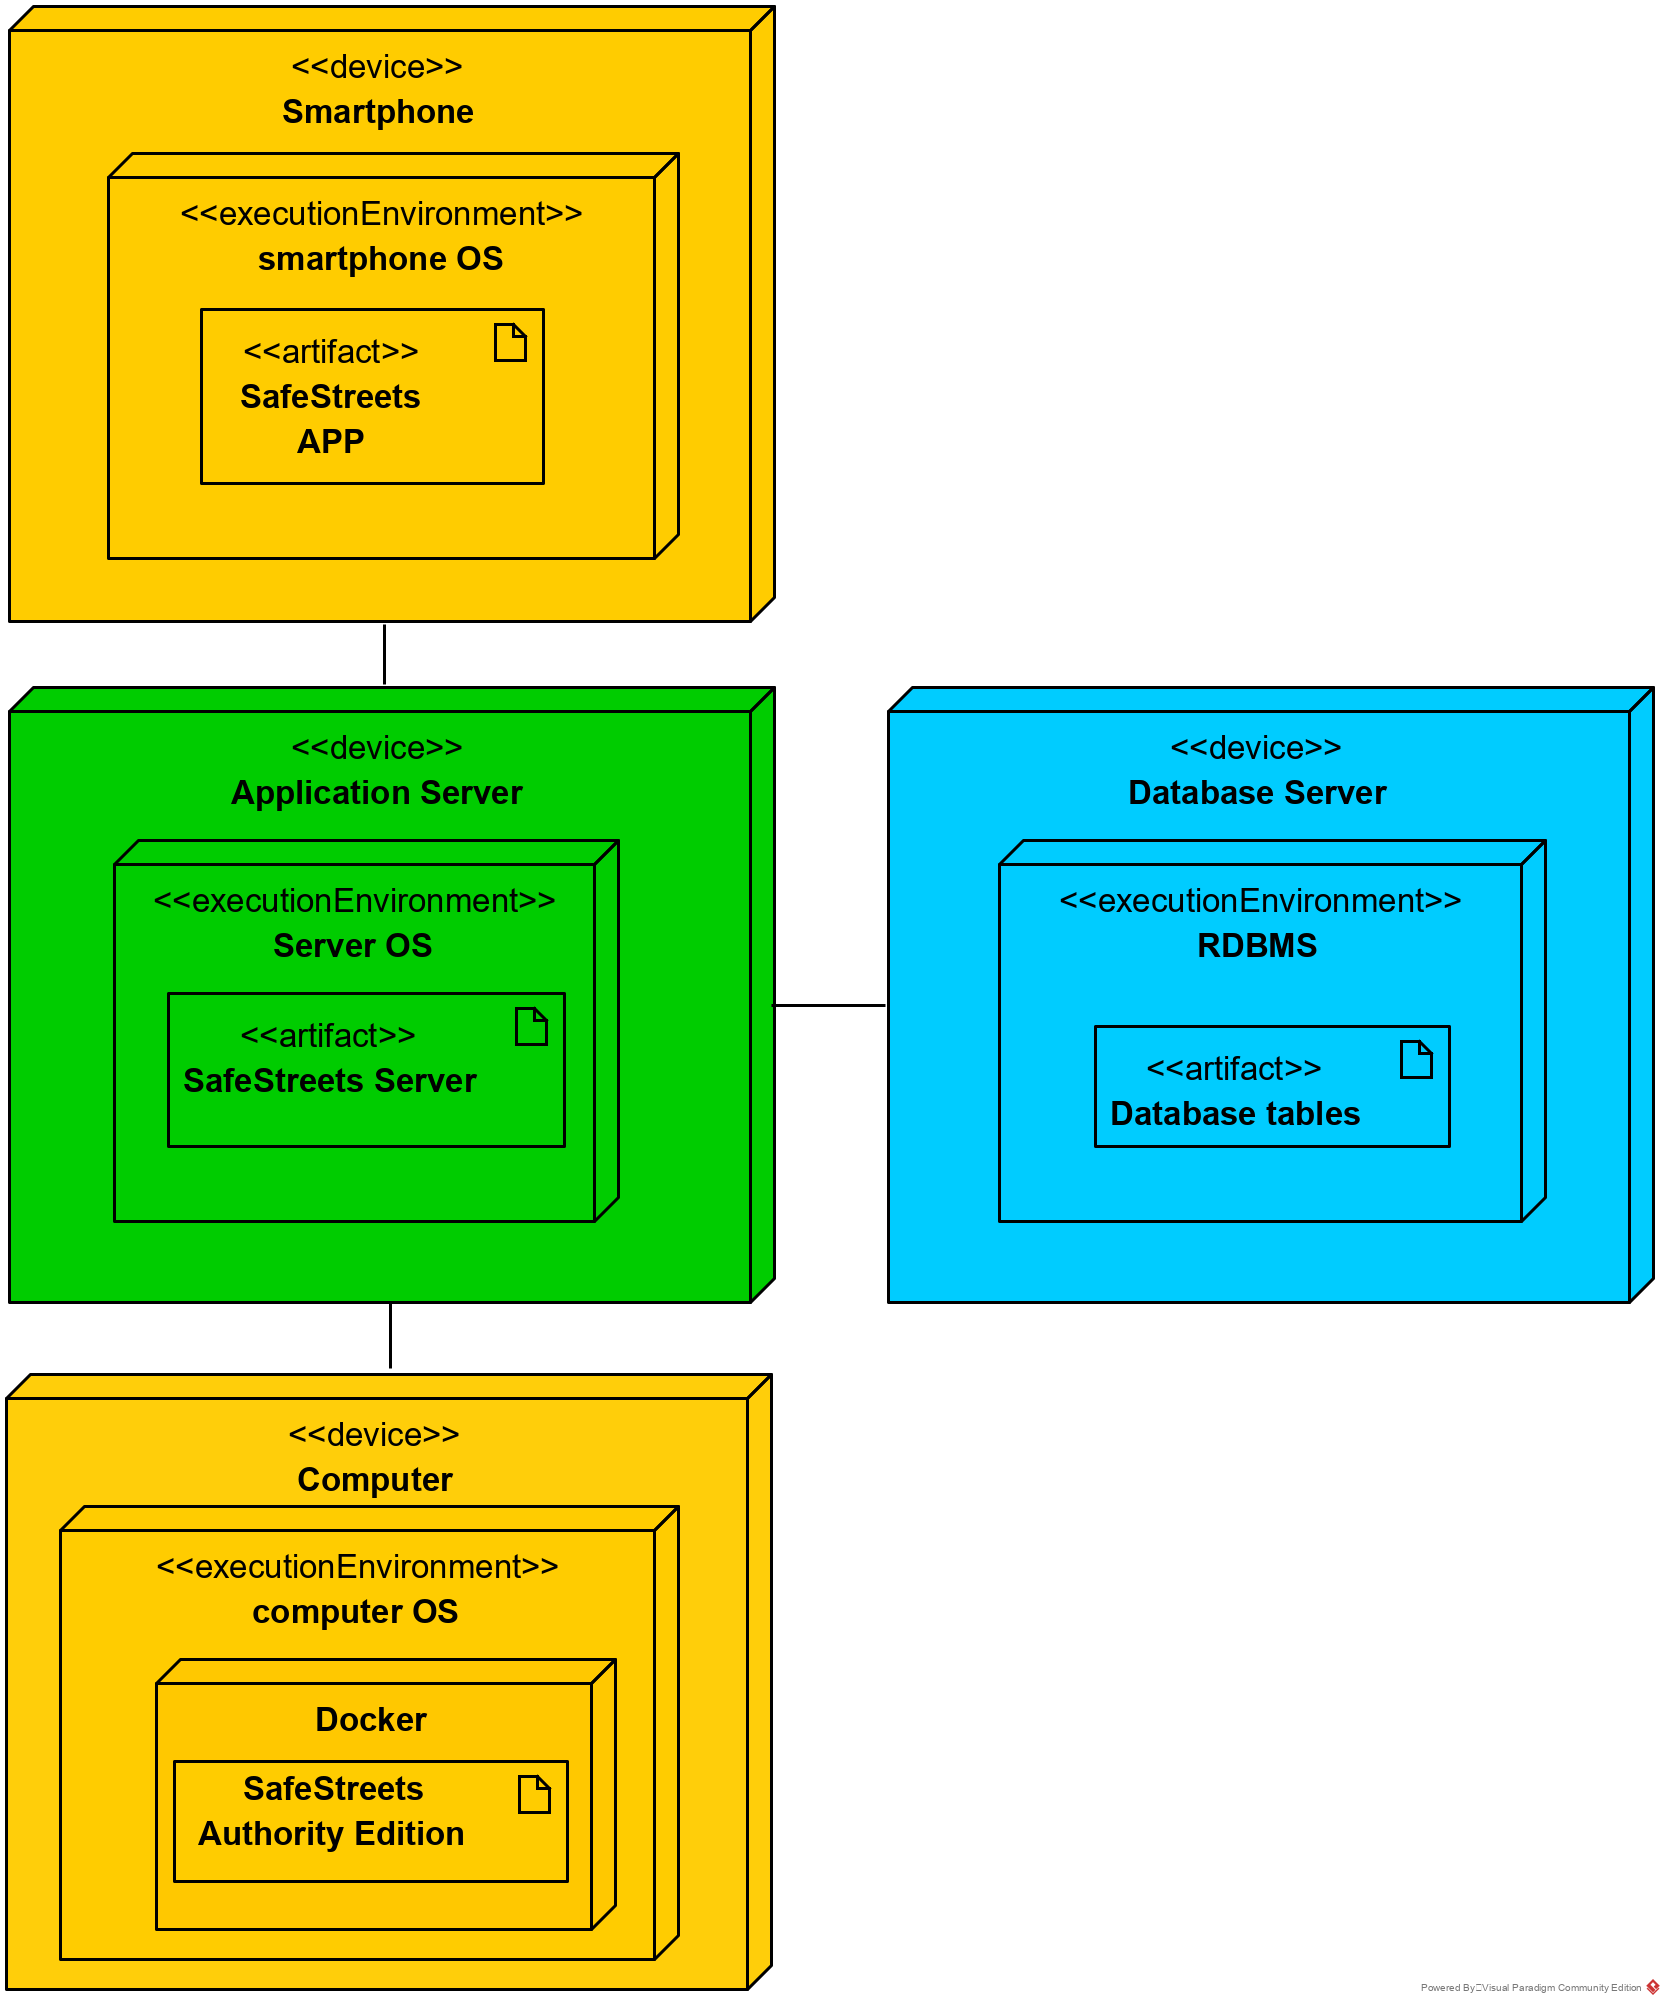
\includegraphics [scale=0.8] {diagrams/deployment_view.png}
			\caption[Deployment View]{Deployment view}
			\label{fig:deployment_view}
		\end{figure}
	
   		SafeStreets App is executed on smartphones and the application is available for the two most popular mobile operative systems: iOS and Android.
   		The smartphone is the device in which both the SafeStreets App view and the SafeStreets App back-end are placed, so it contains the first two logic layers that are the presentation and the application one.\\
   		The smartphone can communicate with SafeStreets Server to execute all the SafeStreets services such as sending a report or browsing through statistics.\\
   		SafeStreets AE is distributed only to authorities that collaborate with SafeStreets. In this context, the application is executable only on computers located in authorities' stations. This type of application is distributed into a (\href{https://www.docker.io}{Docker container}). In this way, the app can be installed on any operating system (more precisely, on any OS for which Docker is available) and the developers of SafeStreets doesn't have to care about the OS on which the app will be executed.\\
   		The reason why the AE is different from the simpler App is that authorities are allowed to make additional and more complete requests to the system and so, a desktop interface and a powerful hardware is better to manage all these requests and to make longer working sessions.\\
   		\\
   		SafeStreets Server is installed on an application Server using preferably a Linux operative system. The Docker middleware is not exploited here, so to have better performance. Moreover, for the server, the possibility of supporting multiple OS is not as relevant as for SafeStreets AE. The server has to manage and forward all the requests in the system and it represent the only way for individuals to retrieve information from the SafeStreets database.\\
   		\\
   		The Database Management System is installed on a non-specific type of server. One possible suggestion is to define it in MongoDB that provides a several number of advantage in terms of security, performance and scalability.\\
   		Other kind of DBMS are also allowed. The key aspect is that the database structure must be relational to satisfy the functionalities required by the system that need a fixed data structure to return specific kind of information or it needs to aggregate related information to make the server able to generate suggestions.
		
		\clearpage
		\subsection{Component interfaces}
		This section describes the methods exposed by each interface that allows the communication between SafeStreets Server and the clients. These interfaces were already briefly shown in the component diagram of figure \ref{fig:component_diagram}.\\
		Information exchanged through these interfaces is standardized with respect to the following class diagram.\\
		
		\begin{figure}[H]
			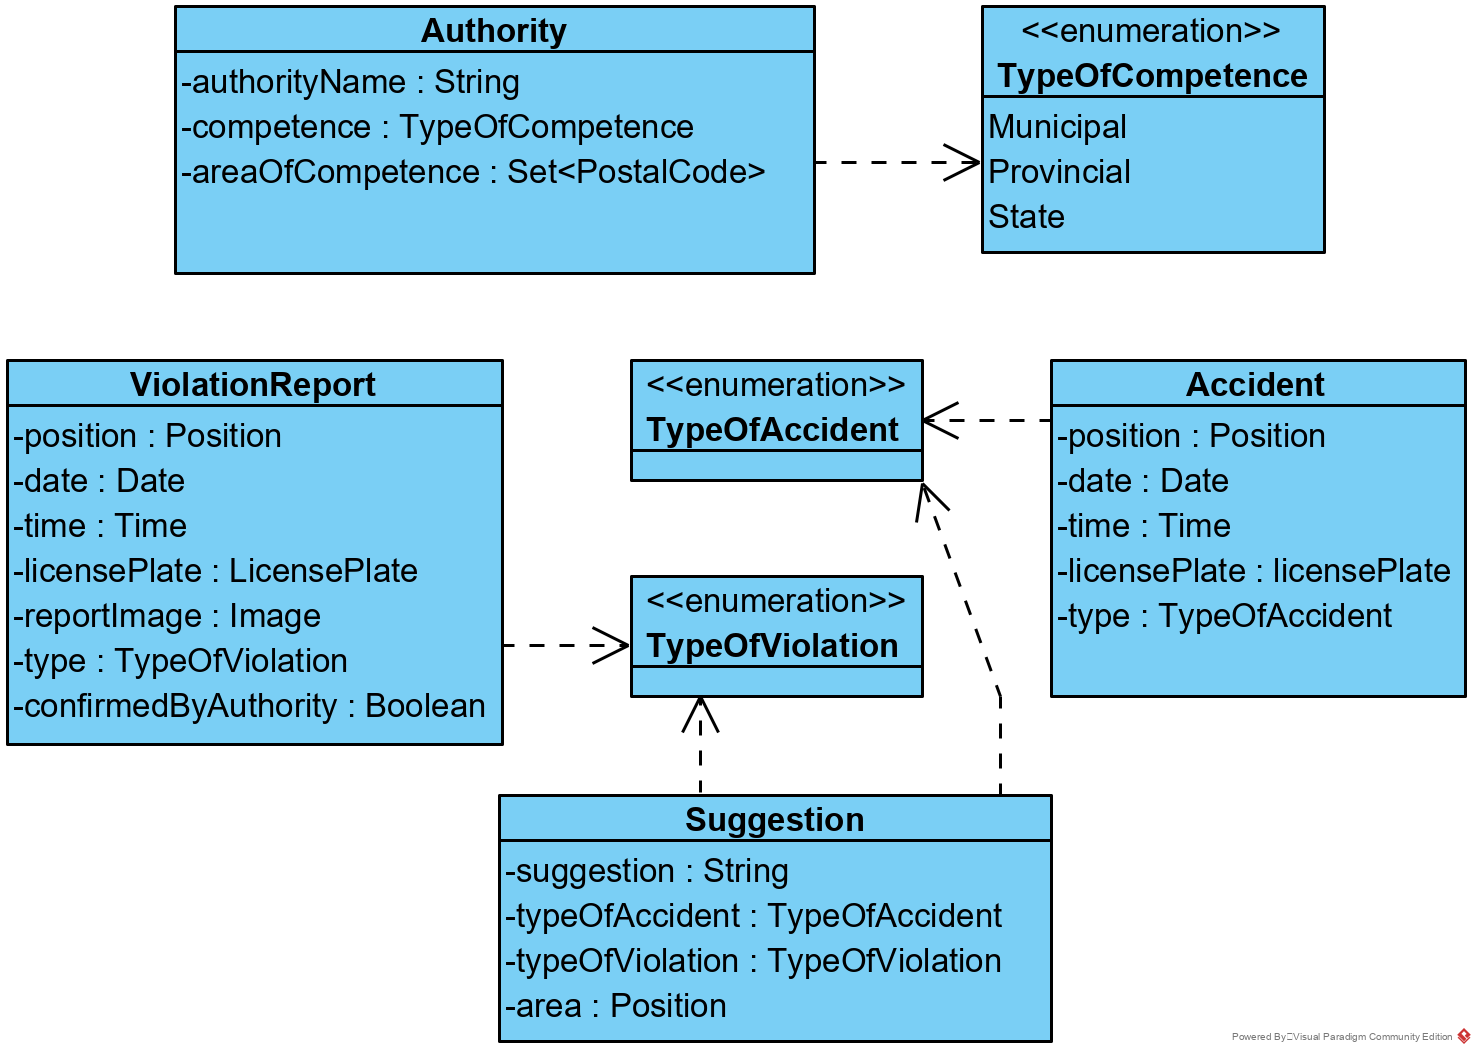
\includegraphics {diagrams/class_diagram.png}
			\caption[Class diagram]{Class diagram}
			\label{fig:class_diagram}
		\end{figure}
	
		The class diagram represents only the classes considered fundamental to understand the operation of SafeStreets. In any case, the classes referred to without providing an explicit declaration - for example the "LicensePlate" class - have a name that effectively expresses their meaning.\\
		\\
		A list of the interfaces follows. For each interface, all the methods it displays are pointed out. For each method, the necessary input parameters and outputs are indicated.\\
		Every interface is exposed by the server to the clients. Therefore, the names of the methods have been chosen from the point of view of the server.\\
		
		\begin{itemize}
			\item \textbf{Anonymous data}\\
				Opportunely combining calls to the following two methods, SafeStreets App can retrieve all the information then used to do data-mining or to show statistics. Notice that SafeStreets App will receive information that doesn't include images or license plates, so it is not possible, being useless, to specify these parameters in the method calls.
				\begin{itemize}
					\item{getCompleteViolationReports}\\\\
					\begin{tabular}{l | l}
						\textbf{Input} & \textbf{Output}\\
						\hline
						positions: Set(Position) & requestedViolationReports: Set(ViolationReport) \\
						dates: Set(Date) &\\
						times: Set(Time) &\\
						types: Set(TypeOfViolation) &\\
						onlyConfirmed: Boolean &\\
					\end{tabular}\\
					\item{getCompleteAccidents}\\\\
					\begin{tabular}{l | l}
						\textbf{Input} & \textbf{Output}\\
						\hline
						positions: set(Position) & requestedAccidents: Set(Accident) \\
						dates: set(Date) &\\
						times: set(Time) &\\
						types: Set(TypeOfAccident) &\\
					\end{tabular}\\
				\end{itemize}
			\item \textbf{Violation report}\\
				This interface exposes only one method that SafeStreets App uses to send a new violation report to the server. The correctness and the completeness of the violation report has already been checked by the app, so the server doesn't have to check it again and to return something as output.
				\begin{itemize}
					\item{receiveViolationReport}\\\\
					\begin{tabular}{l | l}
						\textbf{Input} & \textbf{Output}\\
						\hline
						newViolationReport: ViolationReport & void\\
					\end{tabular}\\
				\end{itemize}
			\item \textbf{Complete data}\\
				Combining calls to the following methods, SafeStreets AE can retrieve all the information used to do data-mining or show statistics to authorities. The information received also contains license plates and images.
				\begin{itemize}
					\item{getCompleteViolationReports}\\\\
					\begin{tabular}{l | l}
						\textbf{Input} & \textbf{Output}\\
						\hline
						positions: Set(Position) & requestedViolationReports: Set(ViolationReport) \\
						dates: Set(Date) &\\
						times: Set(Time) &\\
						types: Set(TypeOfViolation) &\\
						licencePlates: Set(LicensePlate)&\\
						onlyConfirmed: Boolean &\\
					\end{tabular}\\
					\item{getCompleteAccidents}\\\\
					\begin{tabular}{l | l}
						\textbf{Input} & \textbf{Output}\\
						\hline
						positions: set(Position) & requestedAccidents: Set(Accident) \\
						dates: set(Date) &\\
						times: set(Time) &\\
						licensePlates: set(LicensePlate)&\\
						types: Set(TypeOfAccident) &\\
					\end{tabular}\\
				\end{itemize}
			\item \textbf{Violation report evaluation}\\
				The interface is used to send violation reports to evaluate to an authority, and also by the authority to send the result of an evaluation.
				\begin{itemize}
					\item{sendViolationReportsToEvaluate}\\\\
					\begin{tabular}{l | l}
						\textbf{Input} & \textbf{Output}\\
						\hline
						destinationAuthority: Authority & void\\
						ViolationReportTOEvaluate: ViolationReport &\\
					\end{tabular}\\
					\item{receiveEvaluation}\\\\
					\begin{tabular}{l | l}
						\textbf{Input} & \textbf{Output}\\
						\hline
						evaluatedViolationReport: ViolationReport & void\\
						evaluation: Boolean&\\
					\end{tabular}\\
				\end{itemize}
			\item \textbf{Suggestion}\\
			This interface is used by SafeStreets Server to send suggestions to authorities.
				\begin{itemize}
					\item{sendSuggestions}\\\\
					\begin{tabular}{l | l}
						\textbf{Input} & \textbf{Output}\\
						\hline
						destinationAuthority: Authority & void\\
						suggestions: Set(Suggestion)&\\
					\end{tabular}\\
				\end{itemize}
			\item \textbf{Accident}\\
				This interface is used by an authority to send information about an accident to SafeStreets Server.
				\begin{itemize}
					\item{receiveAccidents}\\\\
					\begin{tabular}{l | l}
						\textbf{Input} & \textbf{Output}\\
						\hline
						newAccident: Accident & void\\
					\end{tabular}\\
				\end{itemize}
		\end{itemize}
	
		\clearpage
		\subsection{Runtime	view}
			In the following section, sequence diagrams for SafeStreets are shown.\\
			\\
			Figure \ref{fig:sd-violationReport} shows a detailed interaction between a user and SafeStreets system, through SafeStreets App, using the violation report functionality.\\
			
			\begin{figure}[H]
				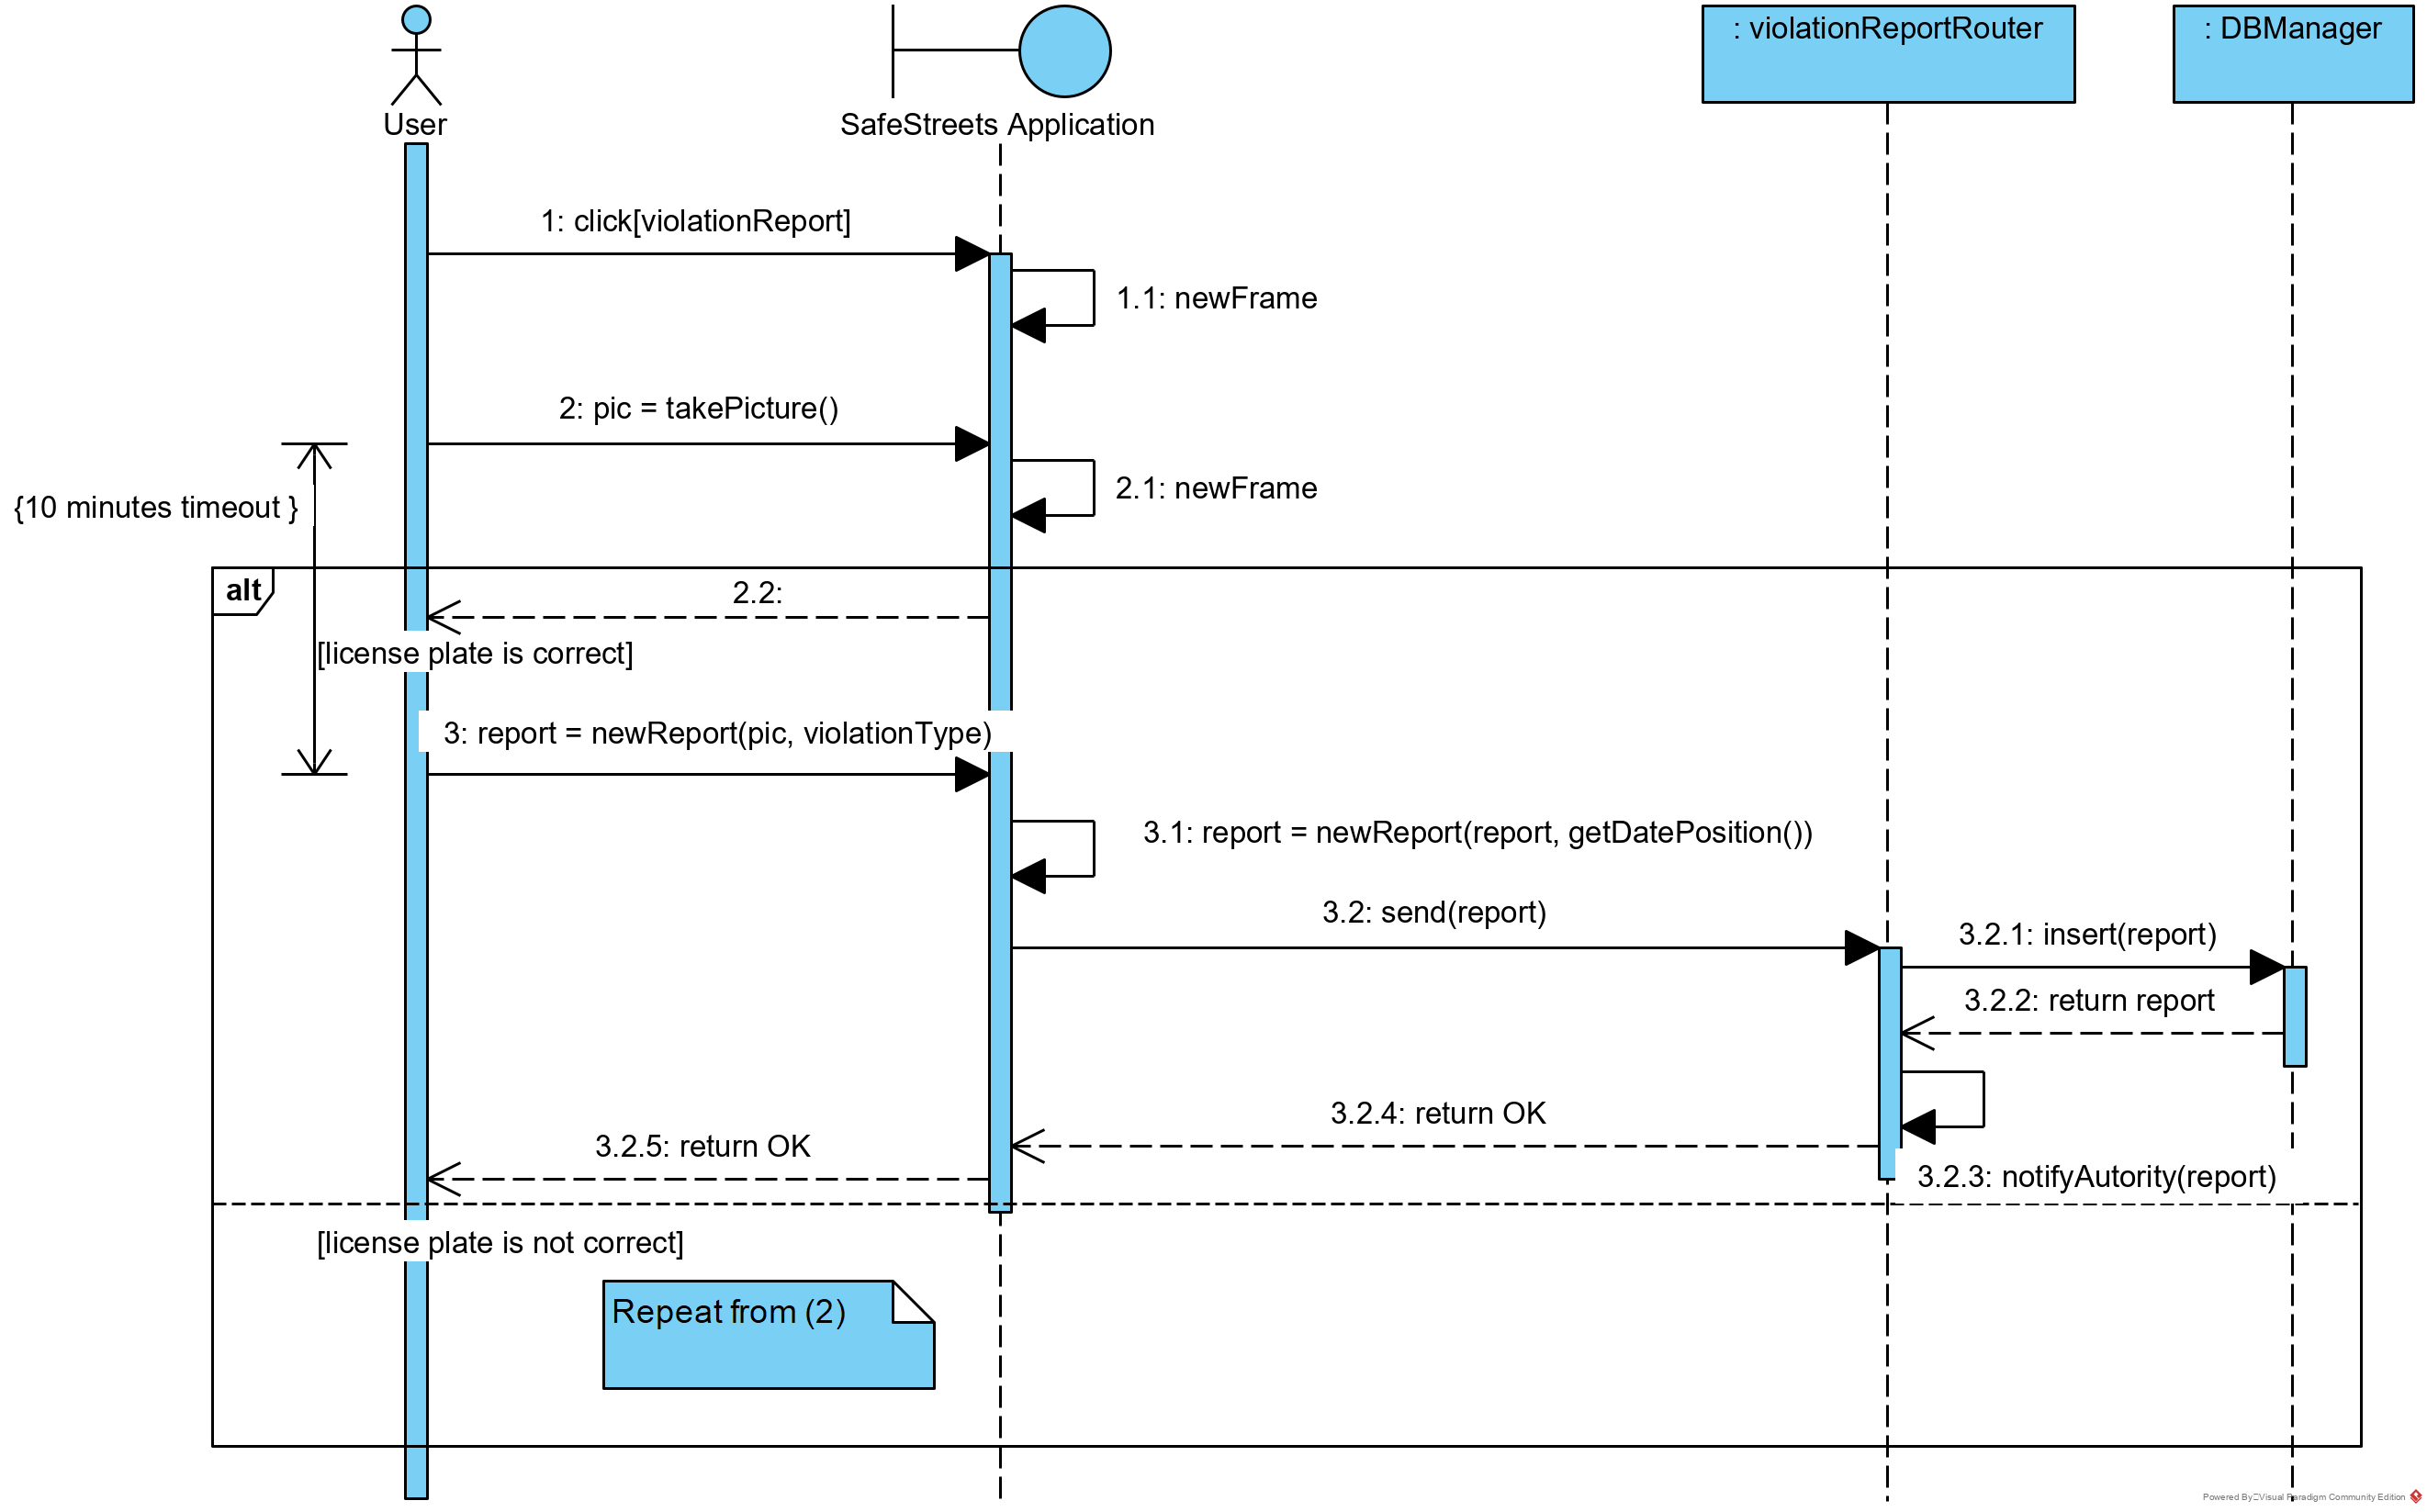
\includegraphics [scale=0.55] {diagrams/DD_SeqD_ViolationReport.png}
				\caption[Sequence diagram]{Sequence diagram for violation reports in SafeStreets AE}
				\label{fig:sd-violationReport}
			\end{figure}
		
			After clicking the apposite menu, the application change its frame and let the user take a photo of traffic violation. Once completed, a countdown of 10 minutes starts: this guarantees that a report could represent an actual violation, so it's not possible neither taking a photo and compile report after a long time, nor upload any photo. SafeStreets Application forces the user to take a photo of violation only through the user interface.\\
			Now, two scenarios can occur: the OCR component of SafeStreets App (described in Figure \ref{fig:component_diagram} and in 2.2.1) recognizes the right license plate or not.\\
			If the license plate read is correct, then the application let the user compile the violation report with remaining information and, before sending it, retrieves data as position and date. 
			The \textbf{:violationReportRouter} forward the report coming from the application to \textbf{:DBManager}.
			This last component stores the report (in pending status) and let the \textbf{:violationReportRouter} notify the authority which operates in the area where the violation occurred. 
			If license plate is either not correct or not detected, then user can repeat the procedure and the report timeout is reset.\\
			
			Authorities evaluate reports as follows in Figure \ref{fig:sd-reportEvaluation}.
			After clicking the apposite menu, SafeStreets AE asks \textbf{:violationReportRouter} to get from \textbf{:DBManager} eventual new reports.\\
			If any reports are retrieved, an authority for each of them can do evaluation, based on photo and information.\\
			Two scenarios have to be managed: if the authority establish that a report is valid ("confirmed"), then \textbf{:violationReportRouter} queries an update of report status to \textbf{:DBManager}; otherwise, if not valid, report should be discarded, so the query asks to delete that report.
			
			\begin{figure}[H]
				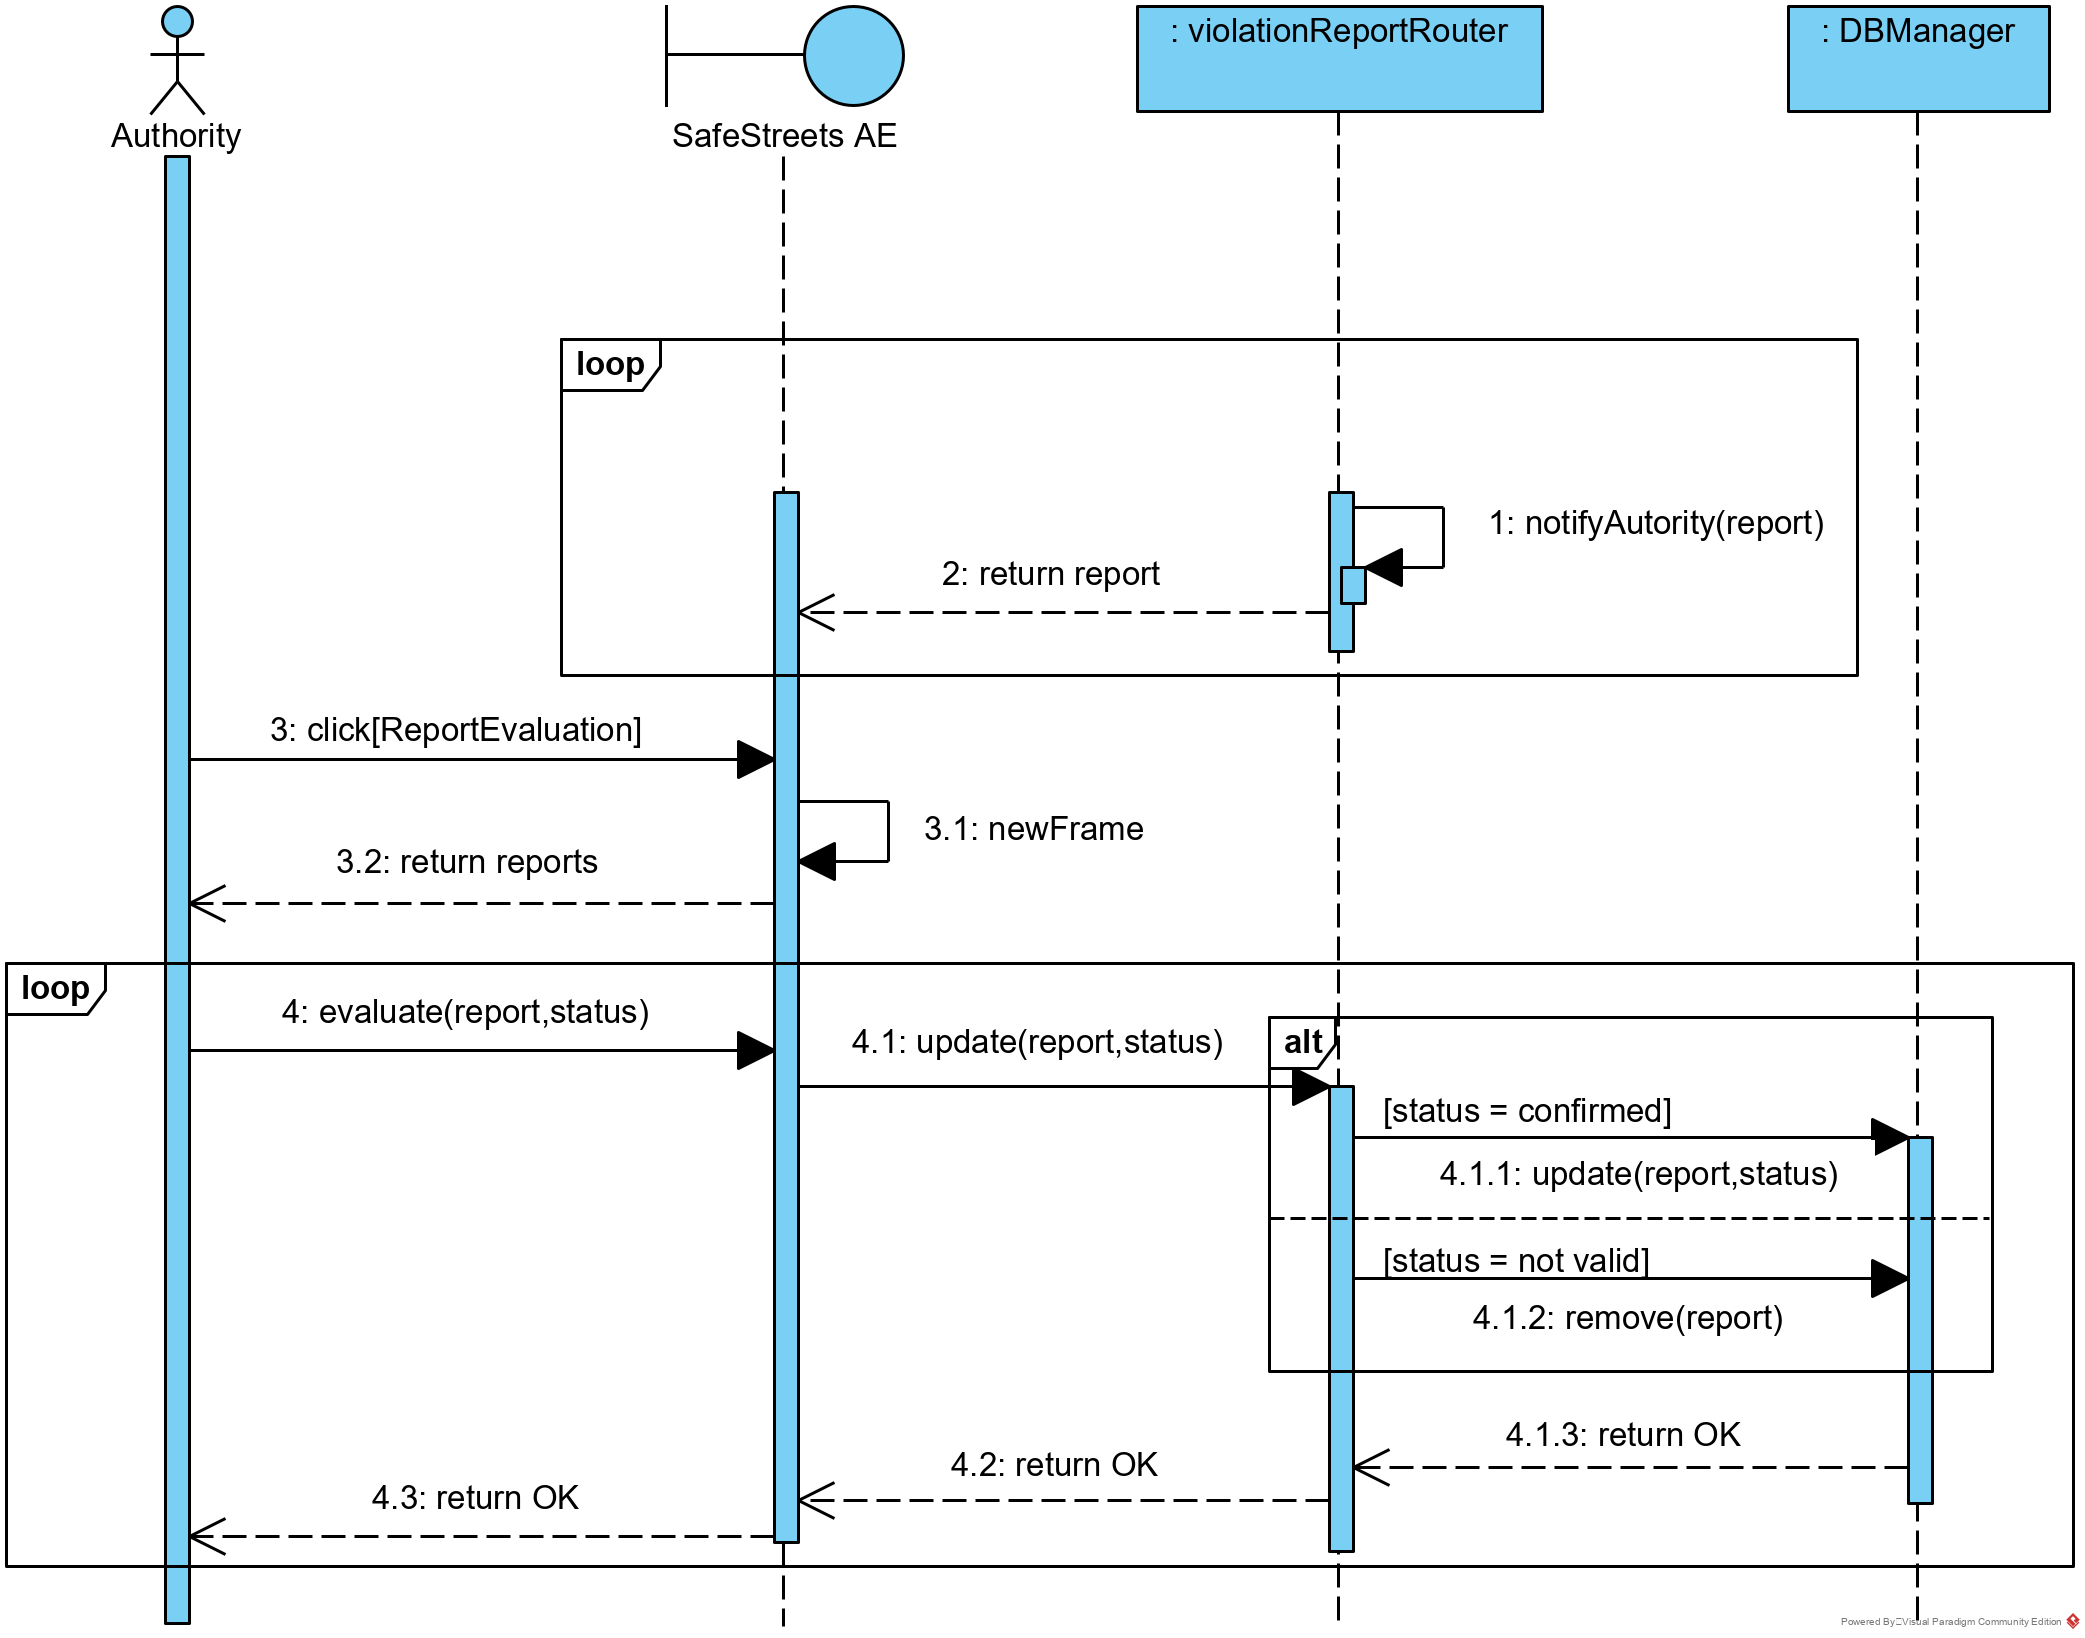
\includegraphics [scale=0.7] {diagrams/DD_SeqD_ReportEvaluation.png}
				\caption[Sequence diagram]{Sequence diagram for report evaluation in SafeStreets AE}
				\label{fig:sd-reportEvaluation}
			\end{figure}
			
			\begin{figure}[H]
				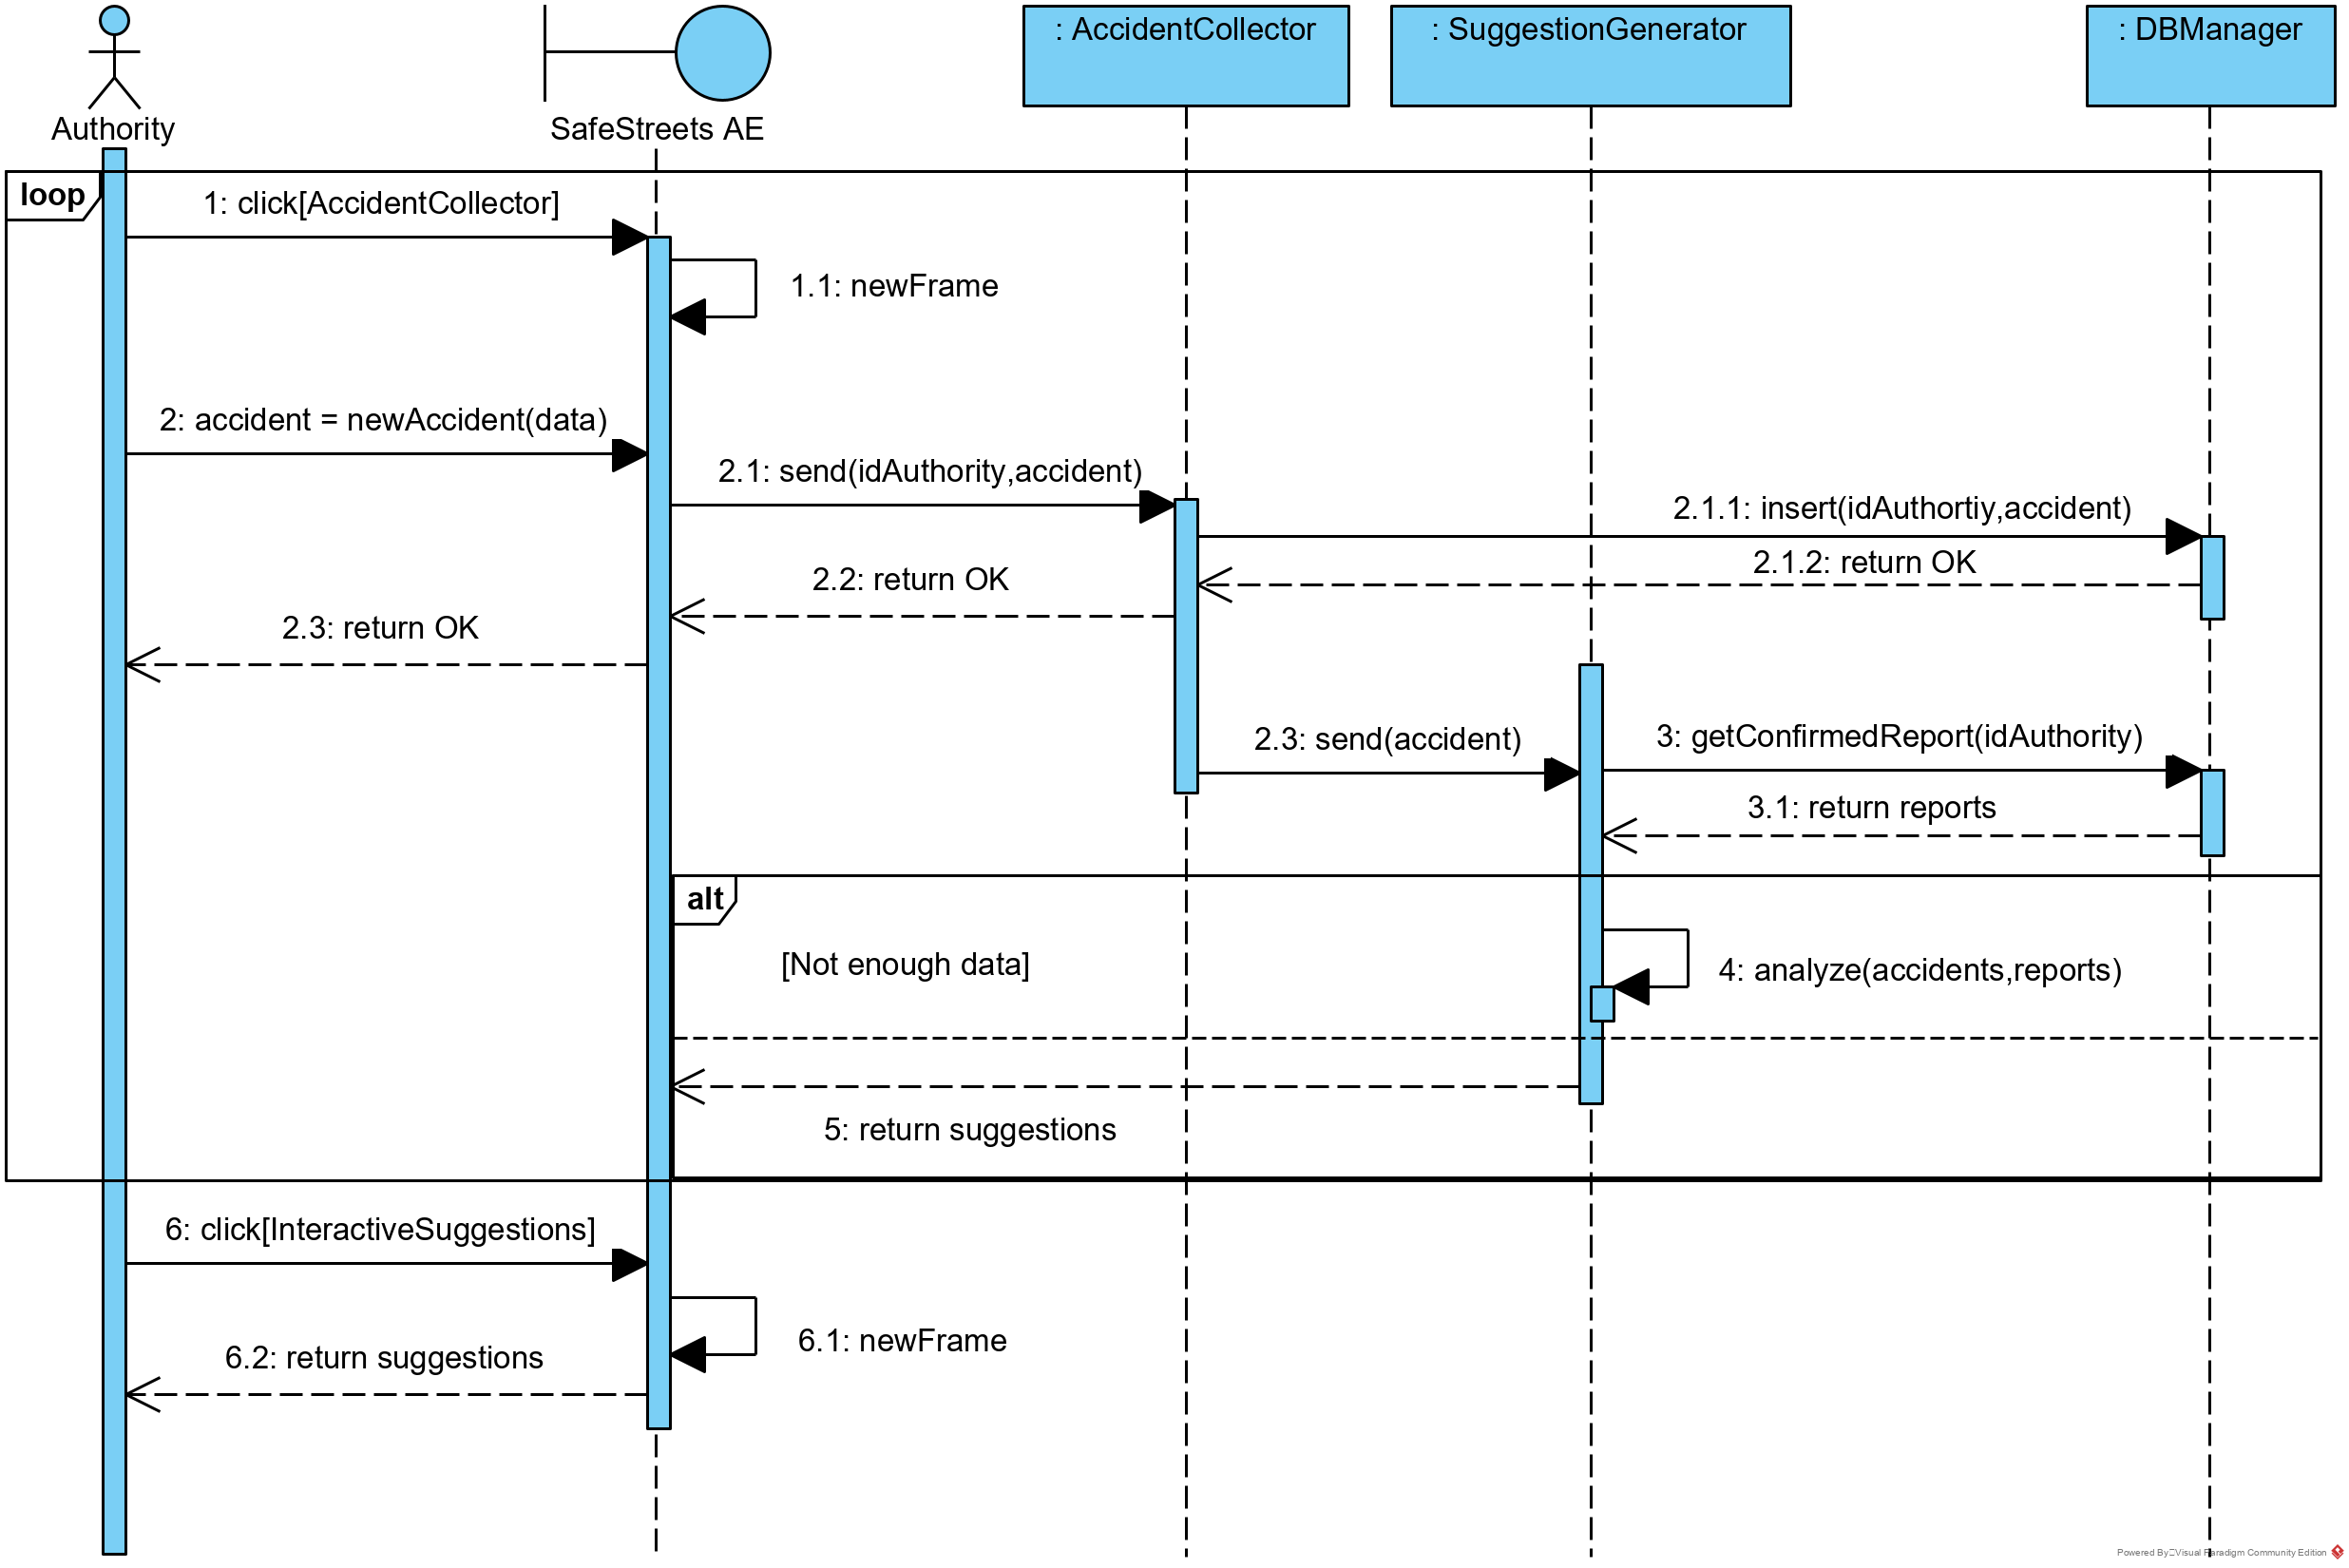
\includegraphics [scale=0.6] {diagrams/DD_SeqD_Suggestions.png}
				\caption[Sequence diagram]{Sequence diagram for interactive suggestions in SafeStreets AE}
				\label{fig:sd-suggestions}
			\end{figure}
		
			A more complex interaction between authorities and SafeStreets system is given in Figure \ref{fig:sd-suggestions}.
			An authority can share with SafeStreets system its data about accidents occurred in its operative area, using the apposite menu. The \textbf{:AccidentCollector} component forwards the accident data from application to \textbf{:DBManager}, which will insert them onto database.\\
			When an authority is notified about new suggestions, it clicks on the apposite menu: SafeStreets AE contacts \textbf{:SuggestionGenerator} component to get suggestions, based on analysis over accident data, stored in the database. 
		
		\clearpage	
		\subsection{Selected architectural styles and patterns}
			\subsubsection{Model-View-Controller (MVC)}
				In order to obtain a clear division between data, user interfaces and software logics, a
				Model–View–Controller (\textbf{MVC}) pattern has been used. MVC is a software design pattern commonly used for developing user interfaces which divides the related program logic into three interconnected elements:
				
				\begin{itemize}
					\item \textit{Model}: the central component of the pattern. It represents the application's data structure, independent from the user interface. It directly manages the data of the application.
					\item \textit{View}: any form of data representation. 
					\item \textit{Controller}: accepts input and converts it to commands for the the model or the view.
				\end{itemize}
				
				One of the biggest advantages of MVC is the possibility to have multiple views of the same information. Thinking about SafeStreets: both users and authorities have their own GUI and different level of details about data.
				This division of concerns makes the application easier to test and maintain: requests first arrive at the controller (or some of them) which binds the model with the corresponding view. 
				In fact, another advantage is the possibility of parallelize application development among workers, such that groups can focus on a fixed part, i.e. model, view and controller.\\
				
				Focusing more on SafeStreets, the MVC division is also observable in Figure \ref{fig:component_diagram}. The back-end of each application, both client and server side, is part of the \textit{controller}; SafeStreets user interfaces represent the \textit{view} and they are just a mean to let users and authorities to communicate with the \textit{model}, information stored in SafeStreets databases.\\
				\\
				Follows an high-level representation of SafeStreets architecture.
				
				\begin{figure}[H]
					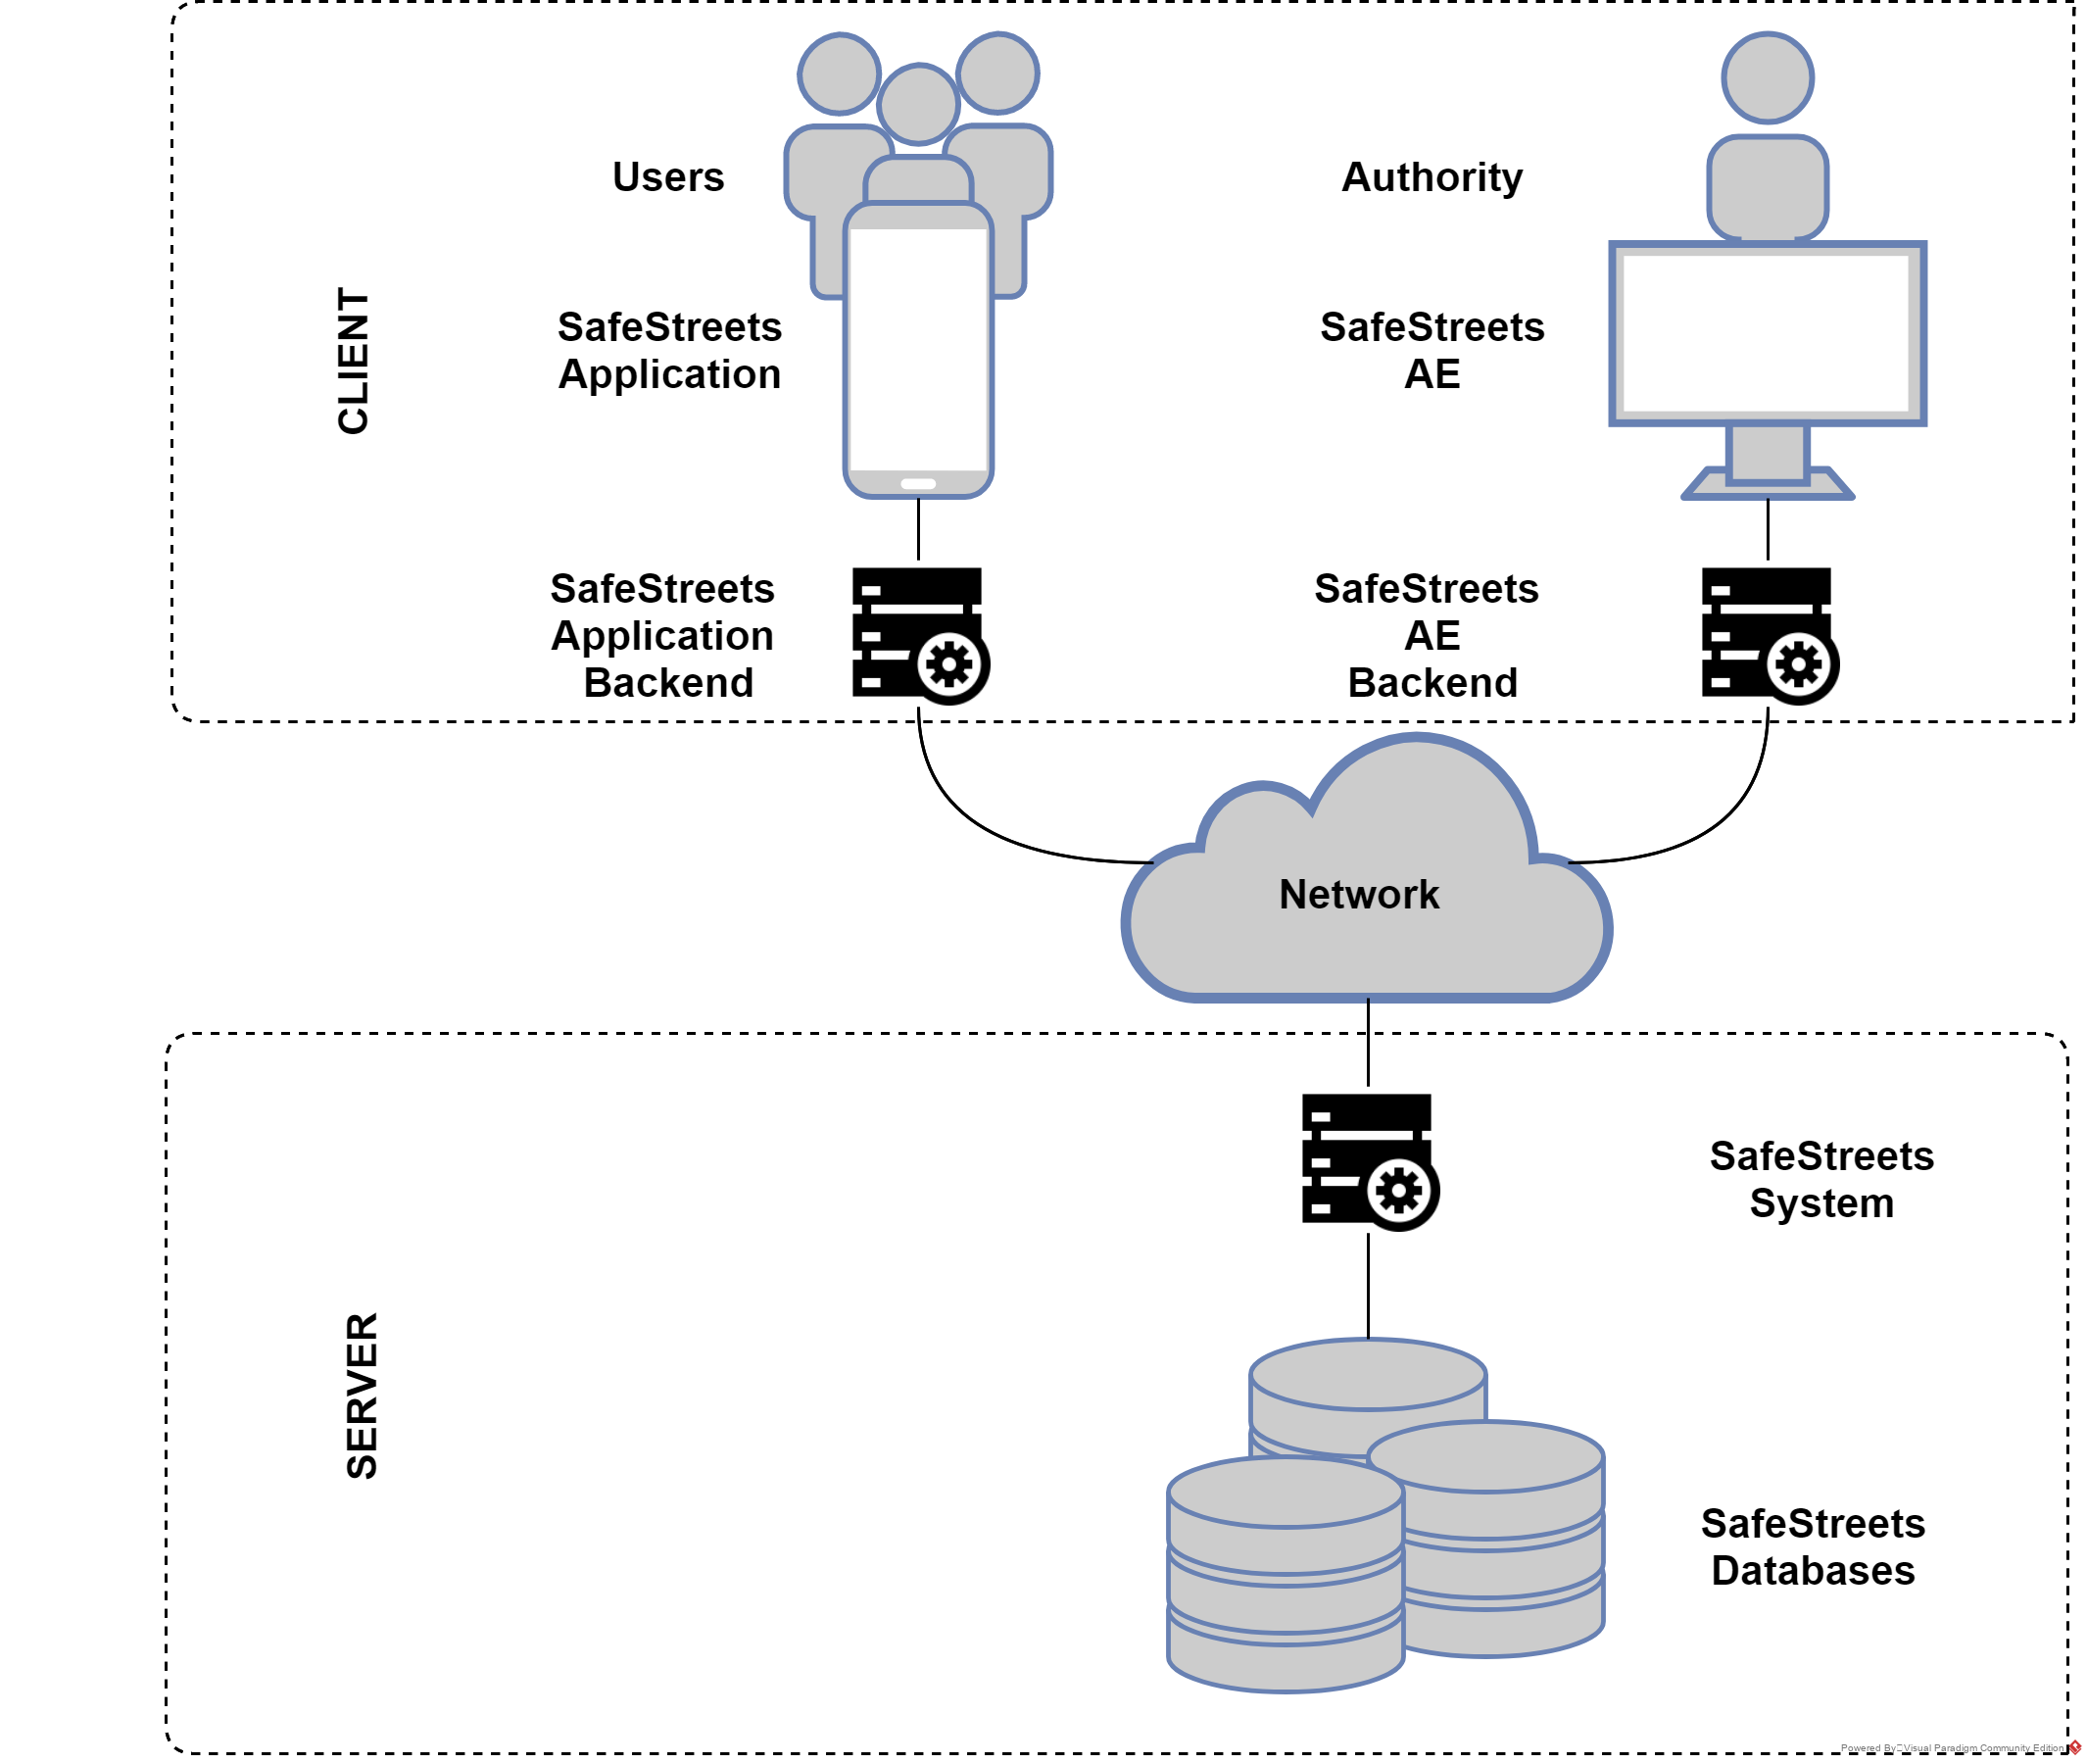
\includegraphics [scale=0.7] {diagrams/tieredArchitecture.png}
					\caption[Architecture]{High-level representation of SafeStreets architecture}
					\label{fig:tieredArchitecture}
				\end{figure}
			
				Figure \ref{fig:tieredArchitecture} gives the idea of two-tiered architecture on which SafeStreets is based: clearly, clients are not \textit{thin}, because they don't have only a presentation layer in their application.
				In fact, with \textit{fat} or \textit{thick} clients there is no need for continuous server communications (e.g. violation reporting for users involve locally an OCR algorithm to verify a correct reading of license plate, without contacting the server generating more workload).
			
			\subsubsection{RESTful web services}
				SafeStreets system doesn't need to exchange, with individuals, complex objects or computations. Basically, there's an exchange of simple objects, easy to format (e.g. in strings, text, file).\\
				In this way, SafeStreets retrieves requests from individuals and returns responses via HTTP, following \textbf{REST} principles.\\
				\textbf{REST} is a software architectural style that defines a set of constraints to be used for creating Web services, in order to provide interoperability between systems on the Internet. 
				
				\begin{figure}[H]
					\centering
					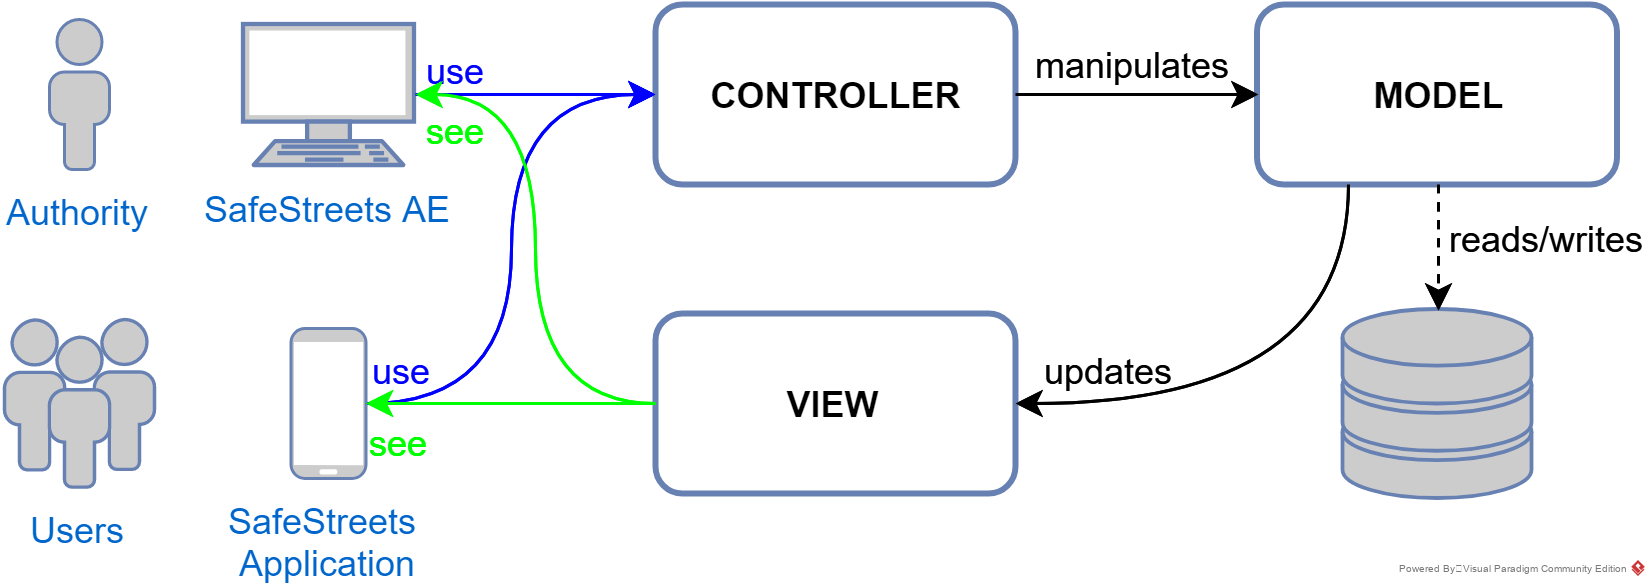
\includegraphics[width=1\textwidth]{diagrams/REST.png}
					\caption[RESTful web services]{RESTful web services}
					\label{fig:RESTful web services}
				\end{figure}

				RESTful Web services allow the requesting systems to access and manipulate textual representations of Web resources by using a uniform and predefined set of \textit{stateless} operations: the client-server communication is constrained by no client context being stored on the server between requests. Each request from any client contains all the information necessary to service the request and the session state is held in the client.\\
				
				A resource is an item of interest, exposed to the clients. In SafeStreets context, examples of resources can be violation reports, accidents or suggestions for authorities.\\
				Every resource is referred in requests using a \textit{URI}, a string of characters that unambiguously identifies the resource.
		
	\clearpage	
	\section{User Interface Design}
		To give an approximate idea of how the interfaces of the application should appear, some mockups, both for SafeStreets Application and SafeStreets AE, have been given in \href{run:d:../DeliveryFolder/RASD1.pdf}{RASD} [Section 3.1.1].\\ 
		In order to express the relations among pictures in RASD [3.1.1], here it will be illustrated a pair of UX Diagrams.\\
		\\
		Functionalities have been represented with different colours, while "Welcome Screen" and "Main Menu" (in purple) are basically the first graphical approach to the app, in particular "Main Menu" contains the menu voices at its right.
		Each functionality has an own sub-flow: black dotted lines represent optional navigation from a screen to another one; blue dotted lines simply refers to the possibility to go back through screens until "Main Menu" is reached.
		
		\begin{figure}[H]
			\centering
			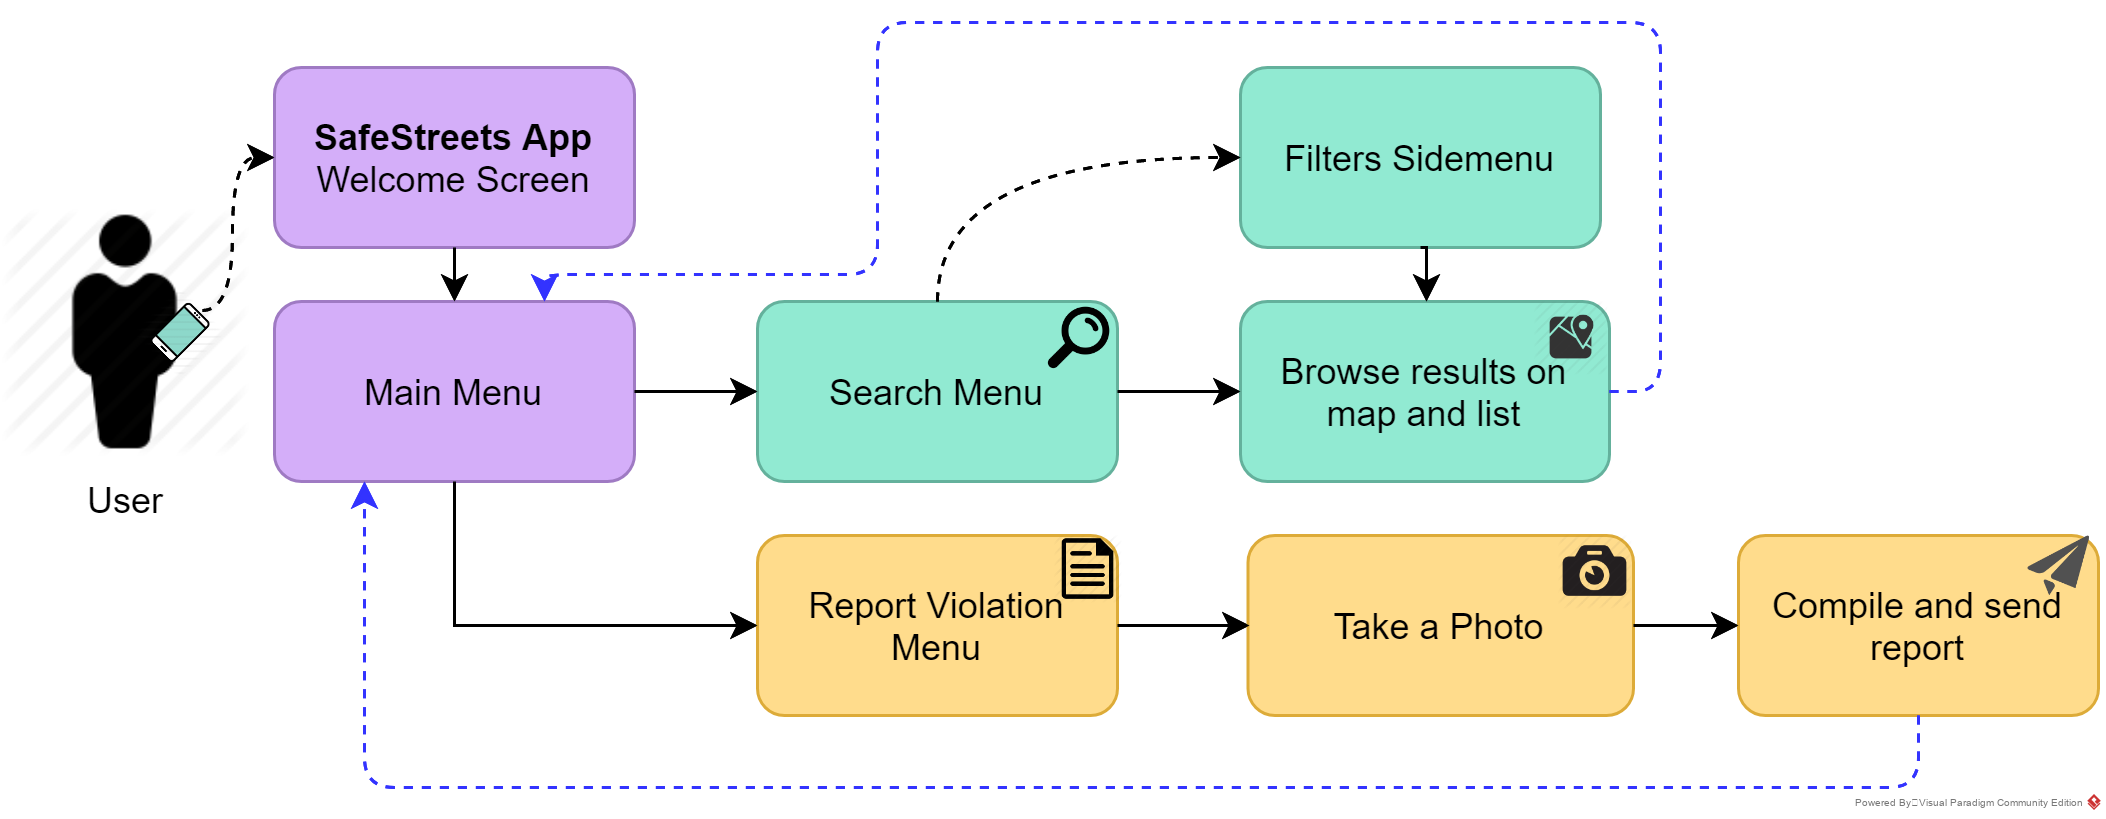
\includegraphics[width=1\textwidth]{diagrams/UXSafeStreetsApp.png}
			\caption[User Experience diagram for SafeStreets App]{User Experience diagram for SafeStreets App}
			\label{fig:UX_SSApp}
		\end{figure}
	
		Figure \ref{fig:UX_SSApp} shows the possibilities given to users, in order to navigate in SafeStreets application. A user can, for instance, select the "Search Menu" to browse all traffic violations reported in an area, showed in a map and listed together in a list.
		Moreover, optionally, a user can improve its research swiping right a side menu in which he can select some filters: the result of research filtered will be shown as the previous modalities, i.e. in the map with a list.
	
		\begin{figure}[H]
			\centering
			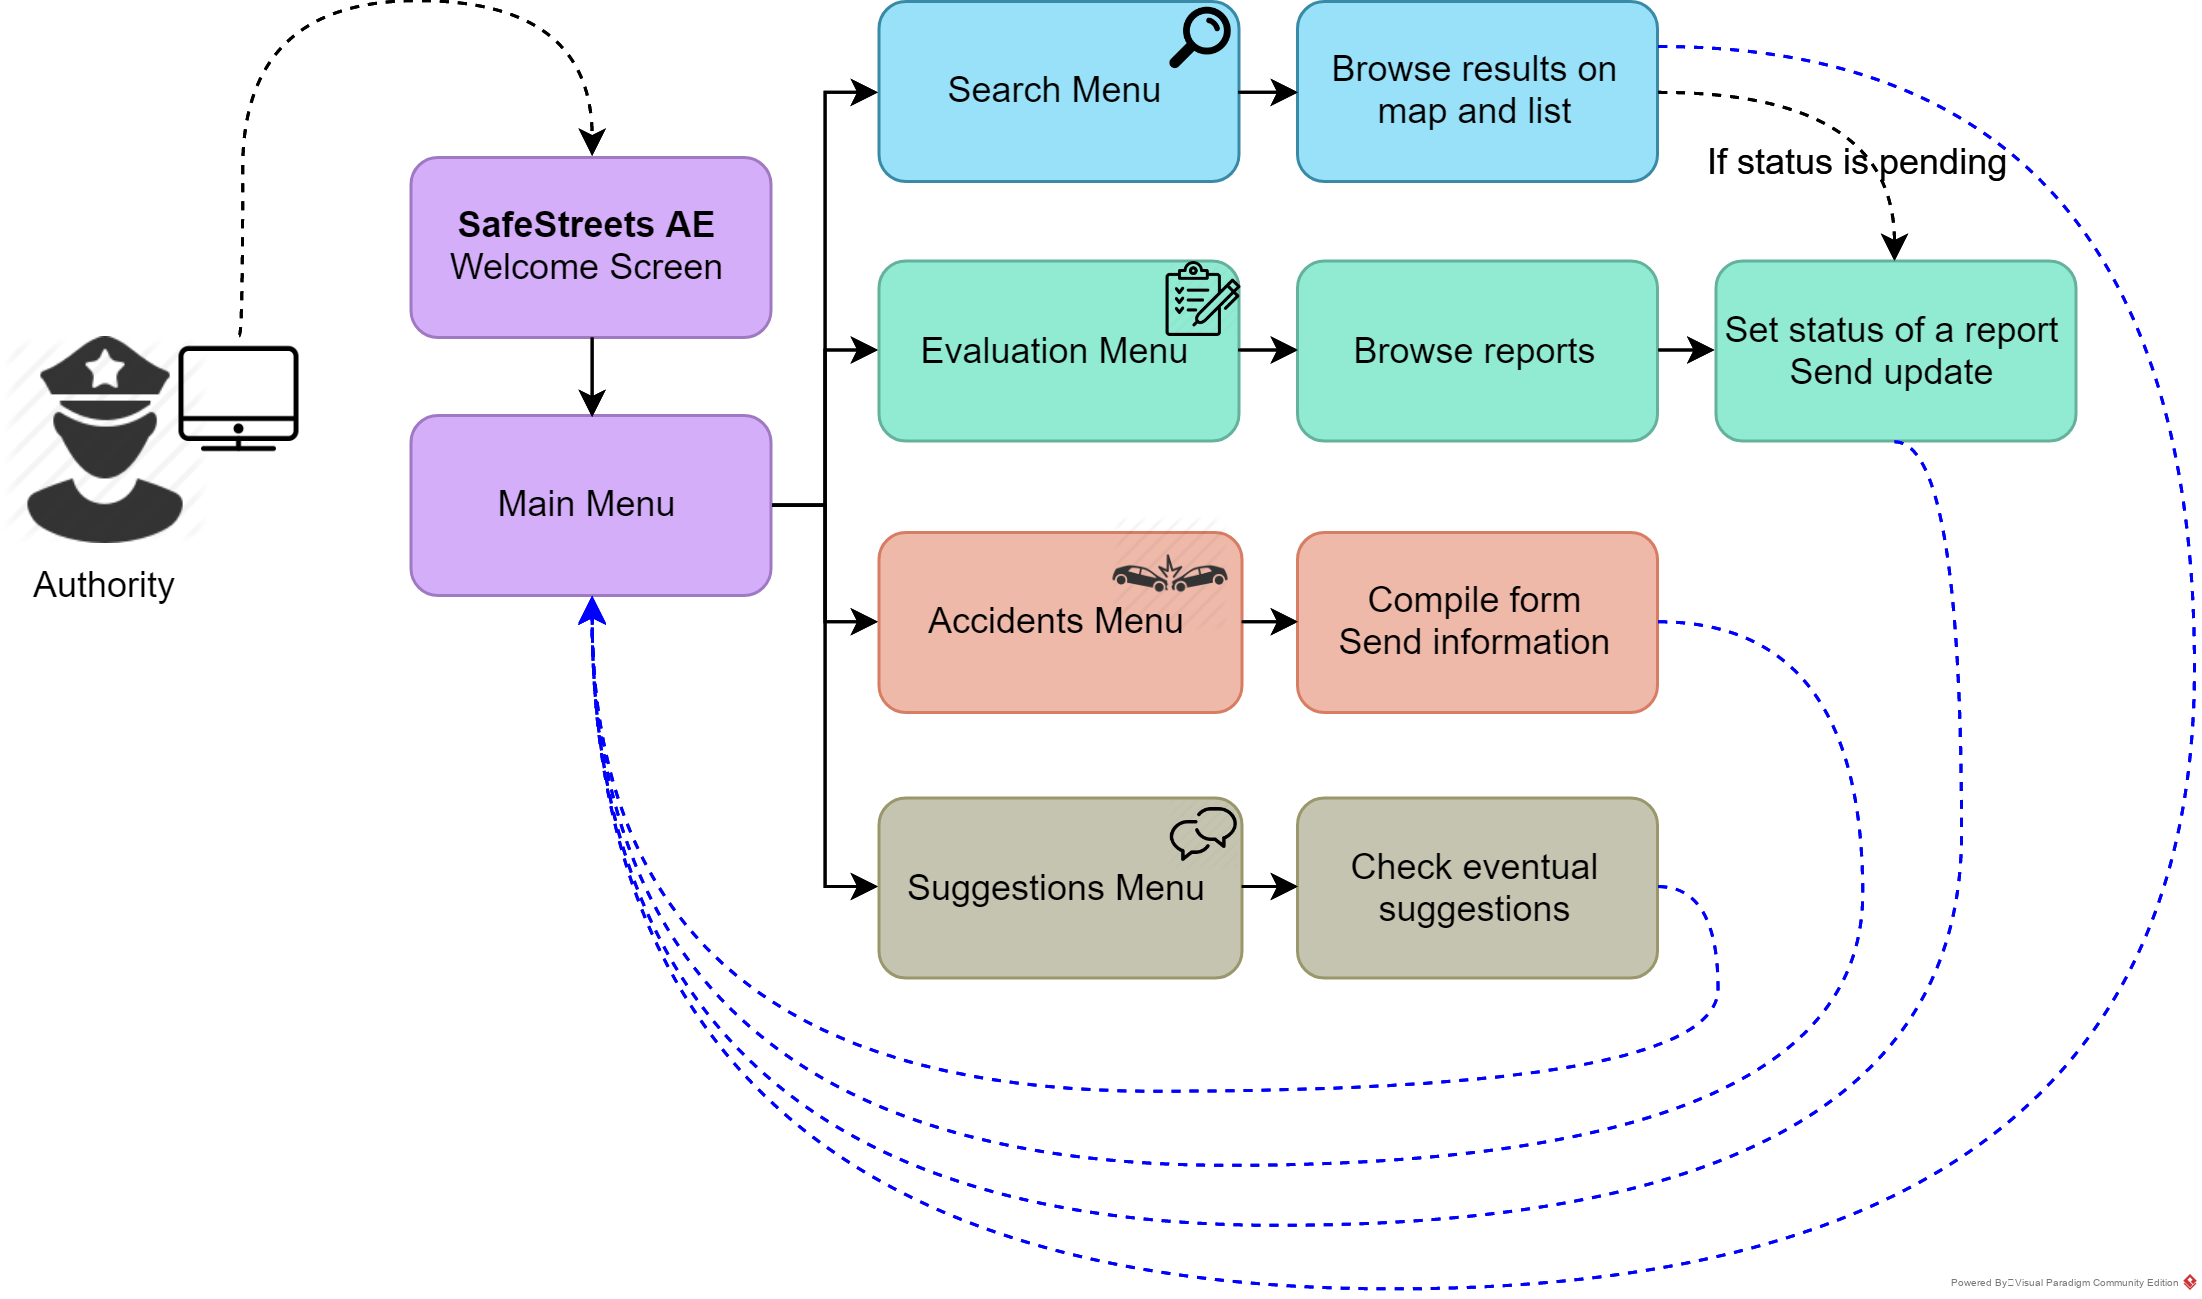
\includegraphics[width=1\textwidth]{diagrams/UXSafeStreetsAE.png}
			\caption[User Experience diagram for SafeStreets AE]{User Experience diagram for SafeStreets AE}
			\label{fig:UX_SSAE}
		\end{figure}
	
		Figure \ref{fig:UX_SSAE} is the user interface flow, designed for authorities who use SafeStreets AE.\\
		Similarly as in figure \ref{fig:UX_SSApp}, here is shown how authorities can explore the offered features. In particular, there's an optional flow which jumps from a result of a research to the "Evaluation" functionality: when an authority browse in a map (using "Search Menu") all traffic violations reported, it can both read information about a particular report and go to evaluation of the same report if and only if its state is pending. In this case, authorities can immediately decide if a report is correct or not valid.
		
	\clearpage	
	\section{Requirements Traceability}
		In this section is shown how the requirements specified in RASD are mapped
		to the design components defined in this document.
		\begin{itemize}
			\requirement{1} The user report must be of one of the type of violation defined by SafeStreets.
			\begin{itemize}
				\item Violation Report Manager
			\end{itemize}
			\requirement{2} The report image must show the license plate of the offender.
			\begin{itemize}
				\item Violation Report Manager
			\end{itemize}
			\requirement{3} The user must insert the picture of the violation.
			\begin{itemize}
				\item Violation Report Manager 
			\end{itemize}
			\requirement{4} The user must complete the report before the expiration of the report timeout.
			\begin{itemize}
				\item Violation Report Manager
				\item Timeout Manager
			\end{itemize}
			\requirement{5} The OCR algorithm must detect one license plate in the report image.	
			\begin{itemize}
				\item Violation Report Manager
				\item OCR
			\end{itemize}
			\requirement{6} The APP must detect automatically position and date.
			\begin{itemize}
				\item Violation Report Manager
			\end{itemize}
			\requirement{7} Every violation report sent to server must be filled in all its fields.
			\begin{itemize}
				\item Violation Report Manager
				\item Violation Report Router
			\end{itemize}
			\requirement{8} The SafeStreets client must show all and only the information required by the individual.
			\begin{itemize}
				\item User data-mining
				\item Authority data-mining
				\item Data-mining Manager
			\end{itemize}
			\requirement{9} Every individual can browse the map.
			\begin{itemize}
				\item User data-mining
				\item Authority data-mining
			\end{itemize}
			\requirement{10} Every individual can see statistics in map.
			\begin{itemize}
				\item User data-mining
				\item Authority data-mining
			\end{itemize}
			\requirement{11} Every individual can define filters for the research.
			\begin{itemize}
				\item User data-mining
				\item Authority data-mining
				\item Data-mining Manager
			\end{itemize}
			\requirement{12} Every authority can see advanced statistics in map (including sensitive information).
			\begin{itemize}
				\item Authority data-mining
				\item Data-mining Manager
			\end{itemize}
			\requirement{13} Every authority can define advanced filters for the research (including sensitive information).
			\begin{itemize}
				\item Authority data-mining
				\item Data-mining Manager
			\end{itemize}
			\requirement{14} The information about accidents must be of one of the type defined by SafeStreets.
			\begin{itemize}
				\item Accident Manager
			\end{itemize}
			\requirement{15} Information about accidents occurred must include all the information required by SafeStreets.
			\begin{itemize}
				\item Accident Manager
				\item Accident Collector
			\end{itemize}
			\requirement{16} Every accident reported by a registered authority is consistently saved into the SafeStreets database.
			\begin{itemize}
				\item Accident Collector
				\item Db Manager
			\end{itemize}
			\requirement{17} Every violation reported to SafeStreets is consistently saved into SafeStreets database.
			\begin{itemize}
				\item Violation Report Router
				\item Db Manager
			\end{itemize}
			\requirement{18} SafeStreets must be able to generate suggestions, based on accidents and confirmed violation reports.
			\begin{itemize}
				\item Db Manager
				\item Suggestion Generator
			\end{itemize}
			\requirement{19} Every authority must receive suggestions only referred to its operative area.
			\begin{itemize}
				\item Suggestion Generator
				\item Suggestion Receiver
			\end{itemize}
			\requirement{20} An authority receives a report if and only if that report is related to a position covered by that authority (i.e. the postal code of the position of the violation report is assigned to that authority)
			\begin{itemize}
				\item Violation Report Router
				\item Violation Report Evaluator
			\end{itemize}
			\requirement{21} When a registered authority confirms a violation report, that confirmation is consistently stored into the server.
			\begin{itemize}
				\item Violation Report Router
				\item Violation Report Evaluator
				\item Db Manager 
			\end{itemize}
			\requirement{22} A violation report rejected by a registered authority is removed from SafeStreets database.
			\begin{itemize}
				\item Violation Report Router
				\item Violation Report Evaluator
				\item Db Manager
			\end{itemize}
		\end{itemize}
			
	\clearpage	
	\section{Implementation, integration and test plan}

		\subsection{Order of implementation}
		We define a precise order of implementation for the various components of SafeStreets ecosystem. To have a complete view of the components, please see the diagram of figure \ref{fig:component_diagram}.\\
		First of all, "DB manager" must be implemented: it manages the interaction between the server and the database, providing query and definition functionalities that are fundamental for the other components.\\
		After that, the components are grouped by the functionality they implement. These groups are sequentially implemented with respect to the order with which their associated functionality is presented into the project assignment. Inside every group, the order of implementation depends on the physical node in which the component is: first the Server, than the App, AE in the end.\\
		Therefore, the first components to be implemented are the ones related to violation reports. In this group, the component of the server closer to the database is "Violation report router". Then we implement the "violation report manager" on SafeStreets App, with its sub-components "OCR" and "Timeout manager". Finally, "Violation report evaluator" is implemented on SafeStreets AE.\\
		\begin{figure}[H]
			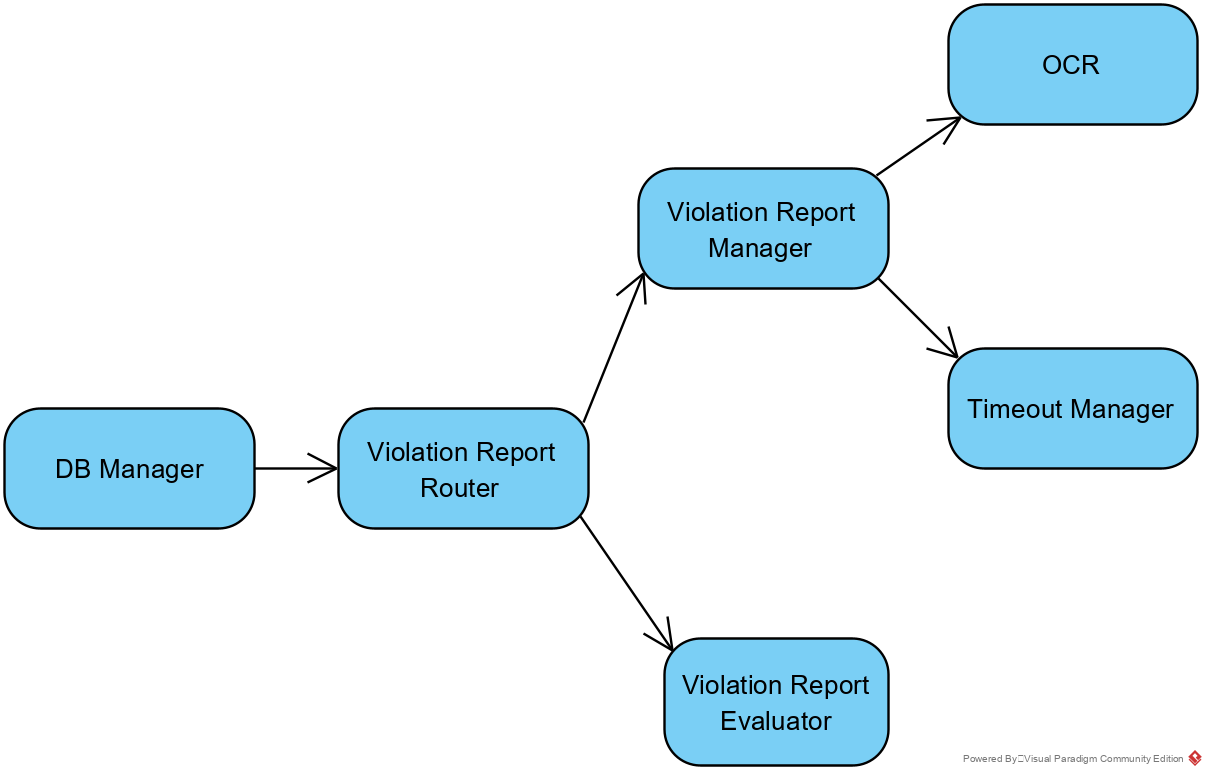
\includegraphics [scale=0.9] {diagrams/report_impltest.png}
			\caption[Report Implementation order]{Report Implementation order}
			\label{fig:report_order}
		\end{figure}
		The second functionality is  about data-mining and statistics. Therefore, in this order, we implement: "data-mining manager" in the server, "user data-mining" in the App, "authority data-mining" in SafeStreets AE.\\
		\begin{figure}[H]
			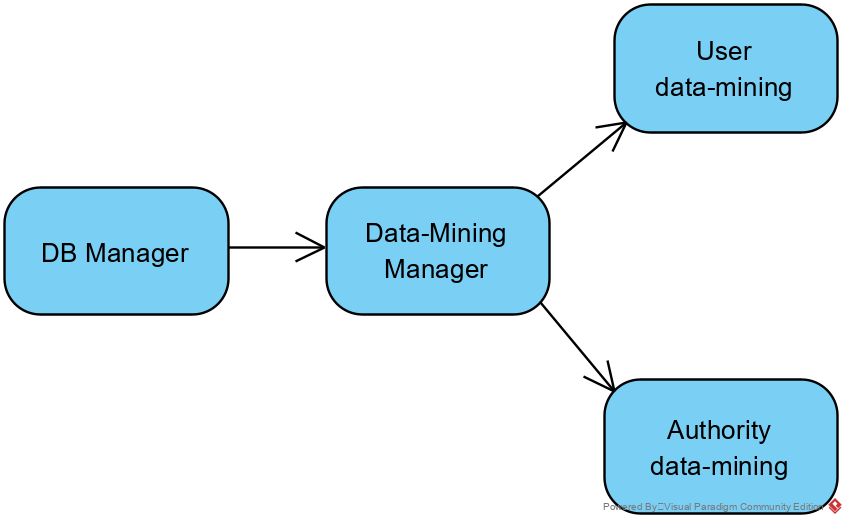
\includegraphics [scale=0.9] {diagrams/datam_impltest.png}
			\caption[Data Mining Implementation order]{Data Mining Implementation order}
			\label{fig:datamining_order}
		\end{figure}
		For "suggestion" functionality, we have "suggestion generator"in the server and "suggestion receiver" in AE.\\
		\begin{figure}[H]
			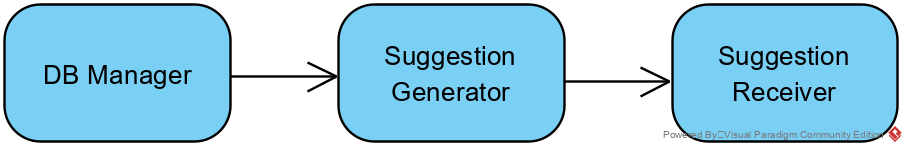
\includegraphics [scale=0.9] {diagrams/suggestion_impltest.png}
			\caption[Suggestions Implementation order]{Suggestions Implementation order}
			\label{fig:suggestions_order}
		\end{figure}
		In the end, for the "accident" functionality, the "suggestion generator" component is implemented, then the "accident manager" on AE.\\
			\begin{figure}[H]
			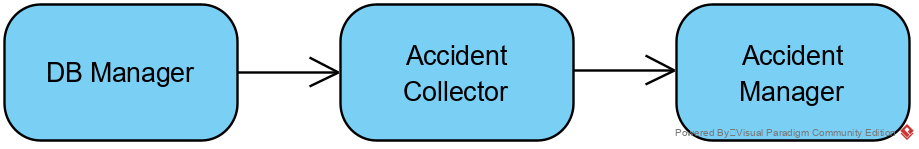
\includegraphics [scale=0.9] {diagrams/accident_impltest.png}
			\caption[Accident Implementation order]{Accident Implementation order}
			\label{fig:accident_order}
		\end{figure}

		\subsection{Integration and testing}
			The implementation of each component must proceed in parallel with its testing phase. As soon as all the components of a given functionality are implemented, an integration test must be performed. Therefore, the order of testing and integration is strictly related to the order of implementation.\\
			Thanks to the MVC pattern, the view and the controller of each functionality can be implemented in parallel. In fact, as soon as the interfaces between the view and the controller have been defined, these components interact only using such interfaces.\\
			When the view and the controller of the same functionality have been implemented, a test of the entire subsystem that manages that functionality has to be done.\\
			When all the functionalities have been implemented, they must be integrated and tested with respect to the node to which their components belong.\\
			In the end, a global test of SafeStreets must be performed.\\
	
	\clearpage
	\section{Effort Spent}
		\begin{table}[h]
			\centering
			\begin{tabular}{l c}
				\hline\hline
				\multicolumn{2}{c}{\textbf{Team Work}} \\
				\hline
				\textbf{Task} & \textbf{Hours} \\ [0.5ex]
				\hline
				Architectural design & 2  \\
				Discussion about Component and Deployment view & 2 \\
				\hline
				\textbf{Total} & 4  \\
				\hline
			\end{tabular}
			\caption{Time spent by all team members}
			\label{fig:Time spent by all team members}
		\end{table}
		
		\begin{table}[h]
			\centering
			\begin{tabular}{l c l c l c}
				\hline\hline
				\multicolumn{6}{c}{\textbf{Individual Work}} \\
				\hline
				\multicolumn{2}{c |}{\textbf{Nicolò Sala}}  &
				\multicolumn{2}{c |}{\textbf{Sebastiano Quacquarelli}} &
				\multicolumn{2}{c}{\textbf{Simone Ricchiuti}}\\
				\hline
				\textbf{Task} & \textbf{Hours}
				& \textbf{Task} & \textbf{Hours}
				& \textbf{Task} & \textbf{Hours} \\ [0.3ex]
				\hline
				%Nicolò								Sebastiano							Simone
				Component view & 4					& User Interface Design & 3					& Introduction & 2
				\\\hline
				Component interfaces & 4						& Runtime view & 2				& Architectural Design  & 4
				\\\hline
				Test plan & 1					& Architectural style/patterns & 4				    & Scheduling plans  & 2 
				\\\hline
				Requirements & 2				& Requirements & 2 			& Requirements & 2 
				\\\hline
					&			&  & 					& &   
				\\\hline
				&							&  & 				&   &   
				\\\hline
				\textbf{Total} & 11				& \textbf{Total} & 9				& \textbf{Total} & 10
				\\\hline
			\end{tabular}
			\caption{Time spent by each team member}
			\label{fig:Time spent by each team member}
		\end{table}
	
	\clearpage
	\section{References}
		\begin{itemize}
			\item "2019-2020 Software Engineering 2 mandatory project: goal, schedules and rules";
			\item TeXstudio (\url{https://www.texstudio.org}) to edit the LaTeX document;
			\item Visual Paradigm CE (\url{https://www.visual-paradigm.com/}) to create UML and ArchiMate diagrams.
		\end{itemize} 
	
\end{document}
